\documentclass[11pt]{article}
\usepackage[utf8]{inputenc}	% Para caracteres en español
\usepackage{amsmath,amsthm,amsfonts,amssymb,amscd}
\usepackage{multirow,booktabs}
\usepackage[table,xcdraw]{xcolor}
\usepackage{fullpage}
\usepackage[bottom]{footmisc}
\usepackage{caption}
\usepackage{subcaption}
\usepackage{listings}
\usepackage{lastpage}
\usepackage{enumitem}
\usepackage{fancyhdr}
\usepackage{mathrsfs}
\usepackage{wrapfig}
\usepackage{setspace}
\usepackage{calc}
\usepackage{multicol}
\usepackage{cancel}
\usepackage[retainorgcmds]{IEEEtrantools}
\usepackage[margin=3cm]{geometry}
\usepackage{amsmath}
\usepackage{algorithm}
\usepackage{algpseudocode}
\newlength{\tabcont}
\setlength{\parindent}{0.0in}
\setlength{\parskip}{0.05in}
\usepackage{empheq}
\usepackage{framed}
\usepackage[most]{tcolorbox}
\usepackage{xcolor}
\colorlet{shadecolor}{orange!15}
\parindent 0in
\parskip 12pt
\geometry{margin=1in, headsep=0.25in}
\theoremstyle{definition}
\newtheorem{definition}{Definition}
\newtheorem{theorem}{Theorem}
\newtheorem{reg}{Rule}
\newtheorem{exer}{Exercise}
\newtheorem{note}{Note}
\numberwithin{equation}{section}
\numberwithin{theorem}{section}
\numberwithin{definition}{section}

\makeatletter
\newcommand{\chapterauthor}[1]{%
  {\parindent0pt\vspace*{-20pt}%
  \linespread{1.1}\large\scshape#1%
  \par\nobreak\vspace*{5pt}}
  \@afterheading%
}
\makeatother

\lstset { %
    language=C++,
    backgroundcolor=\color{black!5}, % set backgroundcolor
    basicstyle=\footnotesize,% basic font setting
}
\title{Computer Vision - Project Report}
\author{Roberto Del Ben - Youssef Ben Khalifa}
\date{\today}
\begin{document}
\maketitle \tableofcontents
\newpage

\section{Introduction}
The goal of this project is to develop a software for the detection and segmentation  of hands. The software is divided in two main modules:
\begin{itemize}
    \item \textbf{Hand detection module}: this module detects the hands inside a given image and draws the corresponding ROI (Bounding Boxes);
    \item \textbf{Hand segmentation module}: this was developed to segment those same hands detected by the previous model.
\end{itemize}

The program is developed using both C++ and Python, the first one is used to process the images using the OpenCV library, extract the dataset and perform
the segmentation, whilst the Python part has the sole purpose of performing the detection using a CNN specifically designed for object detection.

The Hand detection module is based on the use of the \textbf{YOLO}(You Only Look Once) CNN model, which is considered amongst the most efficient object detection algorithms
along with the R-CNN and Fast R-CNN architectures. The goal is to take a known CNN architecture for the YOLO model and train it using the dataset that we will be extracted using
a class that will be implemented into the project.

\section{Image preprocessing [2 hrs]}
\chapterauthor{Roberto del Ben, Youssef Ben khalifa}

The first thing we need in the entire project is to define a pre-processing
pattern for every image. The aim of pre-processing is to transform the image
into a form
that is easier to process, that is, we want to remove as much noise as possible
without losing the important information, while also enhancing the main
features and
improving the general visual representation of the image. This is quite
important, as the processes we will use to perform both the detection and the
segmentation
can be very sensible to additional noise and they are also based on some
features of the image that in some cases may not be noticeable from the raw
image.

For each image we will then apply the following:
\begin{itemize}
    \item \textbf{Bilateral/Gaussian filter}: This filter is a very effective
          way to remove noise from the image;
    \item \textbf{Derivative Filter}: Using an appropriate kernel, we apply a
          spatial filter to the image to enhance small details and edges;
    \item \textbf{Histogram Equalization}: This filter is a very effective way
          to enhance the contrast of the image;
    \item \textbf{Gamma Correction}: It is used to enhance the lighting
          situation in the image, in order to remove dark and light areas that
          hide
          important features of the image,;
\end{itemize}

\section{Dataset creation and extraction [9 hrs]}
\chapterauthor{Youssef Ben khalifa}
We based the project on the EgoHands dataset, which is the same one used for
the benchmarking of the hand detection and segmentation algorithms. The dataset
is available at the following link:

http://vision.soic.indiana.edu/projects/egohands/

since the goal is use a CNN to detect the hands, and as mentioned the
benchmarking will be done partly on the same dataset, to avoid overfitting we
used, in addition to the EgoHands dataset,
the following set of images:

https://www.kaggle.com/datasets/shyambhu/hands-and-palm-images-dataset

The EgoHands dataset was provided with the source RGB images along with the
respective bounding boxes labels as a \textit{csv} file and the masks for the
segmentation. We then processed
the dataset in order to extract the single hand frames from each image, both
segmented and not, for them to be then used for the training of the CNN and
eventually the evaluation for the entire
project.

\subsection{Dataset definition}

To start off, we defined the structure of our dataset in the c++ module, which
can be found the \textit{dataset.h} file: in particular we defined the
\textit{HandMetadata} and \textit{Image}
as follows:

\begin{lstlisting}[]
    class HandMetadata
{
public:
    int PosX;
    int PosY;
    int Width;
    int Height;
    Rect BoundingBox;
    bool isNull;
    bool isInvalid;

    HandMetadata();
    void initBoundingBox();
};

class Image
{
public:
    int id;
    string jpgFileName;
    string maskFileName;
    string csvFileName;
    Mat src;
    Mat mask;
    Mat cannySrc;
    vector<int> coords;
    vector<HandMetadata> handsMetadata;
    vector<Mat> handSrc;
    vector<Mat> handMasks;
    vector<Mat> handFinals;
    vector<Mat> nothands;
    vector<Mat> nothandsCanny;
    vector<Mat> handCanny;

    Image(Mat, Mat, vector<int>);
    void loadCoordinates();
    void cutImage();
    void applyCanny();
    void segmentImage();
    void preProcessImages();
    void cutBackground();
};


\end{lstlisting}

these classed are the ones used throughout the project to help us keep track of
the images and the hands we detect within those same images dataset.
The \textit{HandMetadata} object is in charge of holding all the needed
information about a single detected hand, specifying the boundingBox
coordinates
through the attributes $(PosX, PosY, Width, Height)$ and some flags that will
determine whether the image is read correctly.

The Image class instead holds information about the source image, keeping track
of RGB source image, the mask and the csv associated file containing the box
information;
more importantly in the class is defined a \textit{vector<HandMetadata>} which
is the one attribute that memorize the hands detected in the images. Along with
the attributes
are defined all the necessary methods to read a given dataset.

\subsection{Dataset extraction}
As mentioned earlier, in order to train our CNN we will need all the labelled
samples from the raw dataset that we downloaded. Fortunately the EgoHands
dataset came
pre-packed with some MatLab scripts that allowed us the extract all the images,
the masks and the csv files. After we ran the MatLab scripts we found ourselves
with roughly 5000
rgb images, 5000 grey-scale masks and 5000 csv files. From those images what we
need are the segmented hand images and the RGB images with the bounding boxes,
this heavy
task was accomplished by running the \textit{createDataset()} function defined
in the \textit{Dataset} class (you can find the code in the appendix);

The function writes into separate directories the set of segmented hand images,
the hand images cut using the respecting bounding box coordinates and all the
remaining background images
which will be then lablled as 'notHand'. Those sets are then splitted into
training and test dataset folders using a $0.8-0.2$ split ratio. As the raw
dataset is quite large, the function takes
an additional argument $maxSize$ which is an integer specifying the maximum
size of the dataset we want to extract. Here are some examples of the extracted
images:

\begin{figure}
    \centering
    \begin{subfigure}[b]{0.3 \textwidth}
        \centering
        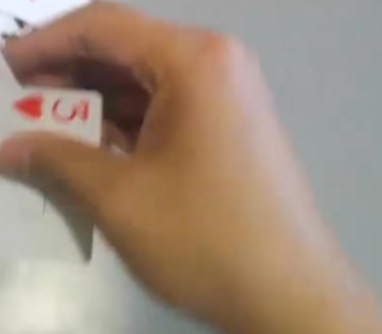
\includegraphics[width=\textwidth]{images/hand/2170.jpg}
        \caption{Hand from Bounding box}
        \label{fig:handBoundeed}
    \end{subfigure}
    \hfill
    \begin{subfigure}[b]{0.3\textwidth}
        \centering
        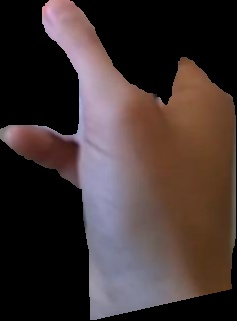
\includegraphics[width=\textwidth]{images/masked/hand231.jpg}
        \caption{Segmented hand}
        \label{fig:three sin x}
    \end{subfigure}
    \hfill
    \begin{subfigure}[b]{0.3\textwidth}
        \centering
        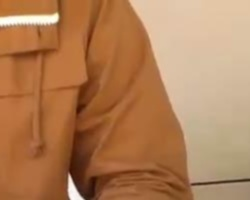
\includegraphics[width=\textwidth]{images/notHand/133.jpg}
        \caption{Background image}
        \label{fig:five over x}
    \end{subfigure}
    \caption{extracted dataset samples}
    \label{fig:three graphs}
\end{figure}

before each image is extracted, we preprocess the source image by applying a
Gaussian blur, a sharpening filter and gamma correction. The preprocessing is
done in order to remove
the noise and to make the image more contrasty, while also adjusting the
lighting.

\section{Hand detection module [8 hrs]}
\chapterauthor{Youssef Ben khalifa}
The hand detection module is composed by two main components:

the fisrt one is developed in C++ acts ad the entry point for the entire
program, and it is responsible for the
fetching the input image and perform the preprocessing on it.

The second partm developed in python, performs the actual detection and
classification of the image given as input argument
by the C++ module.

The detection is based on the usage of a pre-trained YOLO CNN for both the
detection of the ROI in the image and the classification
of those based on two main classes, 'hand' and 'notHand'. The program then for
each hand found writes into a csv file in determined
directory that acts as the connection point between the c++ and python modules:
in that csv file are written the coordinates for each hand found and classified
by the CNN, that same file is then read by the first module and draws the
bounding boxes based on the coordinates written in the csv file. Finally the
input image is
returned with the bounding boxes added.

\subsection{Entry point for the module}

The entire program's entry point is the first c++ module, which requires a
string specifying the input image path:

that image is then read using the $imread()$ method from the OpenCV library and
fed to the $handDetectionModule()$ function the starts the detection:

\begin{lstlisting}

    Mat handDetectionModule(Mat src){
        Mat srcProc;
        Preprocess::equalize(src, src);
        Preprocess::fixGamma(src,src);
        Preprocess::smooth(src, src);
        Preprocess::sharpenImage(src, src);
        imshow("test", src);
        waitKey();
        vector<HandMetadata> hands = detect(src);
        Mat dst = drawROI(src, hands);
    
        return dst;
    }

\end{lstlisting}
this function acts as the actual entry point for the hand detection module, as
it takes as arguments the input image as a \textit{Mat} object and
starts off the detection chain:

the Mat object is preprocessed with a Gaussin filter and a laplacian filter,
then given as argument to the $detect()$ function

\begin{lstlisting}[language = c++]
    vector<HandMetadata> detect(Mat src) {
    imwrite(activeDir + "src.jpg", src);

    string command = pytohnCommand;
    string result = exec(command);
    cout << result << endl;
    vector<int> handROICoords = readCSV(activeDir + "test.csv");

    vector<HandMetadata> hands;
    for(int i=0; i<handROICoords.size(); i+=4){
        vector<int> vec {&handROICoords[i], &handROICoords[i+4]};
        HandMetadata temp = loadHandMetadata(vec);
        hands.push_back(temp);
    }
    
    //cout << "Found " + to_string(hands.size()) + " hand" << endl;
    
    
    return hands;
}
\end{lstlisting}

which starts off the python module for the detection and classification.

\subsection{Python module}
The python module is called using the command line terminal by the detect()
function we had in the c++ module, through the command line no arguments are
passed along,
as the image to process is taken from the \textit{activeDir} folder used as the
connection point between the two modules in which the input image is written by
the
c++ module for the python program to read. As soon as the python module is
loaded, the YOLO CNN model is loaded along with it from the local configuration
files
saved under the directory \textit{python/models/YOLO}:

\begin{lstlisting}[language=python]
    if __name__ == "__main__":

        srcPath = activeDir + "src.jpg"
        detect(srcPath, scoreThreshold)
        print("done")
        quit()
\end{lstlisting}

the $detect()$ function reads the image path and loads it into the YOLO model
to detect.

\begin{lstlisting}[language=python]
    def detect(srcPath):
    src = imread(srcPath)
    #detect ROI for hands for boundingBoxes
    handRoi = detectROI(src)
    rows = []
    for detection in handRoi:
        x, y, w, h = detection
        handFrame = src[x-100:x+w+100, y-100:y+h+100]
        savepath = activeDir + "test.jpg"
        imsave(savepath, handFrame)
        predicetedSrc = cnn.predict(savepath)
        print(predicetedSrc)
        rows.append([x,y,w,h])
    writeCsv(activeDir + "test.csv", rows)
\end{lstlisting}

In the detect method we read the image path and initialize it as a \textit{Mat}
object from the \textit{cv2} library and feed it to the
yolo object through the $detectROI()$ function which returns a vector of
bounding boxes. From those bounding boxes we extract the ROI for each hand and
save it in the
\textit{activeDir} folder as a \textit{csv} file.

\subsection{ROI Drawing and output}
Once the Python module is done writing the coordinates for the bounding boxes
into the \textit{csv} file,
the a callback to the c++ module is done to continue the main execution and
proceed to drawing the bounding boxes:
this last task is achieved through the usage of the $drawROI()$ function. The
function takes as arguments the vector of objects $HandMetadata$ which we
previously
read loaded from the csv file in the $detect()$ function using the following
code:

\begin{lstlisting}
    vector<int> handROICoords = readCSV(activeDir + "test.csv");
    vector<HandMetadata> hands;
    for(int i=0; i<handROICoords.size(); i+=4){
        vector<int> vec {&handROICoords[i], &handROICoords[i+4]};
        HandMetadata temp = loadHandMetadata(vec);
        hands.push_back(temp);
    }
\end{lstlisting}

amongst those line you'll notice a particular method called $readCSV()$, this
is one is the same one we used during the dataset extraction at the beginning
which we can easily recycle to accomplish the task of reading the \textit{csv}
file containing the Hands coordinates. The \textit{vector<HandMetadata> hands}
is then passed along to the \textit{detectROI}; this function return the output
image, again as a \textit{Mat} object, with the bounding boxes drawn in
different colors, one for each hand detected.

\begin{lstlisting}[language = c++]
    Mat drawROI(Mat src, vector<HandMetadata> hands){
    Mat dst = src.clone();
    int colorId = 0;
    int thickness = 2;
    for(auto hand : hands){
        Point p1(hand.PosX, hand.PosY);
        Point p2(hand.PosX + hand.Width, hand.PosY + hand.Height);
        rectangle(dst, p1, p2,
                colors.at(colorId),
                thickness, LINE_8);
        colorId += 1;
        if(colorId == colors.size()) colorId = 0;
    }
    
    return dst;
}

\end{lstlisting}

\subsection{YOLO model}
This is a particular type of CNN which we re-trained on the egohands dataset we extracted at the beginning of the project. It is based on the YOLOv3 architecture, which is a convolutional neural network designed specifically
for object detection and classification:

\begin{figure}[!h]
    \centering
    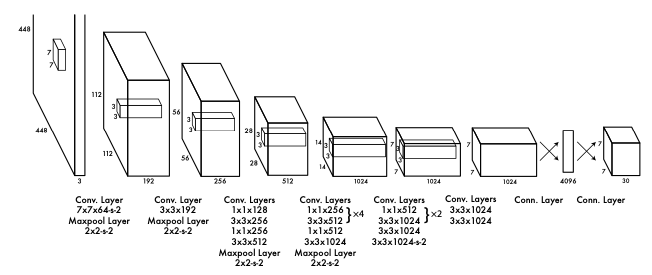
\includegraphics[scale = 0.5]{images/yolo1_net.png}
\end{figure}

in our program we initialize the YOLO object the code line

\begin{lstlisting}[language=python]
    yolo = YOLO('../python/models/yolo/yoloTrained.cfg',
            '../python/models/yolo/yoloTrained.weights', ["hand"])
\end{lstlisting}
in which we specify the class to detect and nothing else. All the other
paramters are already set to the best values in the
YOLO class constructor.

which we found at the beginning of the \textit{main.py} script. The object is
loaded form the class \textit{YOLO.py}
in which we find all the methods needed to initlize the object and perform the
detection. We then defined the model as follows:

\begin{lstlisting}[]
nc: 1
depth_multiple: 0.33
width_multiple: 0.50

anchors:
  - [10,13, 16,30, 33,23] 
  - [30,61, 62,45, 59,119]
  - [116,90, 156,198, 373,326] 

backbone:
  [[-1, 1, Focus, [64, 3]],
   [-1, 1, Conv, [128, 3, 2]],
   [-1, 3, Bottleneck, [128]],
   [-1, 1, Conv, [256, 3, 2]],
   [-1, 9, BottleneckCSP, [256]],
   [-1, 1, Conv, [512, 3, 2]], 
   [-1, 9, BottleneckCSP, [512]],
   [-1, 1, Conv, [1024, 3, 2]],
   [-1, 1, SPP, [1024, [5, 9, 13]]],
   [-1, 6, BottleneckCSP, [1024]],
  ]

head:
  [[-1, 3, BottleneckCSP, [1024, False]],
   [-1, 1, nn.Conv2d, [na * (nc + 5), 1, 1, 0]],
   [-2, 1, nn.Upsample, [None, 2, "nearest"]],
   [[-1, 6], 1, Concat, [1]],
   [-1, 1, Conv, [512, 1, 1]],
   [-1, 3, BottleneckCSP, [512, False]],
   [-1, 1, nn.Conv2d, [na * (nc + 5), 1, 1, 0]],
   [-2, 1, nn.Upsample, [None, 2, "nearest"]],
   [[-1, 4], 1, Concat, [1]],
   [-1, 1, Conv, [256, 1, 1]],
   [-1, 3, BottleneckCSP, [256, False]],
   [-1, 1, nn.Conv2d, [na * (nc + 5), 1, 1, 0]],

   [[], 1, Detect, [nc, anchors]],
  ]
\end{lstlisting}

the same model is then trained using our custom dataset we extracted mostly
from the egohands dataset and some third-party sources, using a dedicated
python script we find in the \textit{yoloV5} folder.
The script outputs two main files: a \textit{.cfg} file containing the
configuration for our CNN, and a \textit{.weights} file containing the weights.
Those files are the ones we find in the \textit{models/yolo} folder
that will be loaded into the python script.

The YOLO model is implemented into the python model through the
\textit{YOLO.py} class we find under the \textit{python} directory, in which we
find along with the constructor for
the class, the \textit{inference()} method:

\begin{lstlisting}[language = python]
    def inference(self, image):
        ih, iw = image.shape[:2]
        blob = cv2.dnn.blobFromImage(
            image, 1 / 255.0, (self.size, self.size), swapRB=True, crop=False)
        self.net.setInput(blob)
        layerOutputs = self.net.forward(self.output_names)
        boxes = []
        confidences = []
        classIDs = []
        for output in layerOutputs:
            for detection in output:

                scores = detection[5:]
                classID = np.argmax(scores)
                confidence = scores[classID]

                if confidence > self.confidence:

                    box = detection[0:4] * np.array([iw, ih, iw, ih])
                    (centerX, centerY, width, height) = box.astype("int")

                    x = int(centerX - (width / 2))
                    y = int(centerY - (height / 2))

                    boxes.append([x, y, int(width), int(height)])
                    confidences.append(float(confidence))
                    classIDs.append(classID)

        idxs = cv2.dnn.NMSBoxes(
            boxes, confidences, self.confidence, self.threshold)

        results = []
        if len(idxs) > 0:
            for i in idxs.flatten():
                # extract the bounding box coordinates
                x, y = (boxes[i][0], boxes[i][1])
                w, h = (boxes[i][2], boxes[i][3])
                id = classIDs[i]
                confidence = confidences[i]

                results.append((x, y, w, h))

        return results
\end{lstlisting}

which takes a \textit{Mat} object as input and returns a list of vector
coordinates $(x,y,w,h)$, that correspond respectively $(x,y)$
coordinates of the top-left corner of the box, its width and height. These
values are returned for each hand detected in the input image.

The hand detection made by the YOLO module is particularly biased by one main
parameter, which is the \textit{confidence}: this determines the
probability of the image analyzed by the module to be a hand. The
\textit{confidence} is set to 0.5 by default, but can be changed in the
constructor of the \textit{YOLO} class.

The main reason for such a low confidence value is the simple fact that we are
interested in detecting one single class label, which is 'hand'. All other
possible labels are considered as
'notHand', therefore not detected. Thus 50\% of the detected labels are hands.

\subsection{Model training}
The training of the YOLO model was done using the \textit{train.py} script, which is found in the \textit{yolo} directory: the script 
can be executed by typing
\begin{lstlisting}[]
    !python train.py --img 416 --batch 32 --epochs 25 
        --data <path to the dataset configuration file> 
        --cfg <path to the model configuration file>
\end{lstlisting} 

in the terminal. The needed file must be \textit{.yaml} files, which we easily converted to from the original \textit{.csv} files 
we got during our dataset extraction using a simple tool found online. 

The training was done using roughly 1000 images per epoch, and a batch size of 32: the training of one single model took about 2.5 hours to complete
running on a local machine with a dedicated GPU. The configuration file are finally saved in the \textit{models/yolo} folder, which we then used 
to perform the detection. In total we attempted the detection using 3 different models, each with different configuration parameters and structures 
and choose the best one based on the evaluation ran on a separate test set extracted using our Dataset class from the c++ module.
Here are the results of the evaluation:
\begin{itemize}
    \item \textbf{Model 1}: training score: 0.988, test score: 0.981;
    \item \textbf{Model 2}: training score: 0.879, test score: 0.872;
    \item \textbf{Model 3}: training score: 0.953, test score: 0.918; 
\end{itemize}

\subsection{Overfitting and Data augmentation}
The main problem we may encounter by using mostly images from the same dataset to train the CNN models is overfitting. This may happen whenever
the training dataset may not be diverse enough, and lead to generating features that work perfectly as long as we work on the same data that come from 
the same source. We can avoid this problem by using data augmentation, which is a technique that allows us to generate various type of images from the 
same images we have in our dataset, by simply applying random transformations, and applying different size rescales onto the images.


\subsection{Usage}
The detection can be done calling the \textbf{handDetectionModule()} function we find in the \textit{main.cpp} source file, which takes as paramters a Mat object representing 
the input image. It return a Mat object with the drawing boxes drawn on top of the input image. If you wish to check the numerical coordinates for the bounding boxes, 
you can directly check the \textit{test.csv} file generated by the python script under the \textit{activeDir} folder.

\subsection{Important Notes}
Note that the only way that the c++ and python module can communicate and work properly together in thought the \textbf{activeDir} directory we find 
the root project folder, so DO NOT DELETE the activeDir, or if you do, recreate it! 

One last thing to note is the python launch command in the \textit{main.cpp} file: you need to adjust it based on your local machine.

\section{Hand Segmentation Module}
\chapterauthor{Roberto del Ben}

\subsection{Coarse segmentation [2 hrs]}
We chose to make a first coarse segmentation based on a range of colors that
skin can have inside images. First of all we consider the \textit{YCrCb} color
space, since in the RGB color space similar colors do not always correspond to
similar values. Then, since this range isn't well defined due to
different illumination sources or camera settings, we used a very large portion
of the \textit{YCrCb} spectrum in order to exclude only very unlikely
combinations. These values came from some researches done in the internet and
validated through the dataset by the following code:

\begin{lstlisting}[language = c++]
    Mat HandsSegmentation::GetSkinMask() {
        int min_cr = 135, max_cr = 180, min_cb = 85, max_cb = 135;
        Mat ycrcb_range, ycrcb_ms_image;
        cvtColor(image, ycrcb_ms_image, COLOR_BGR2YCrCb);
        inRange(ycrcb_ms_image, Scalar(0, min_cr, min_cb), 
                Scalar(255, max_cr, max_cb), ycrcb_range);
    
        Mat mask;
        auto element_type = MORPH_ELLIPSE;
        auto element_size = 6;
        Mat element = getStructuringElement(element_type, 
                        Size(element_size * 2 + 1, element_size * 2 + 1));

        morphologyEx(ycrcb_range, mask, MORPH_CLOSE, element);
    
        return mask;
    }
\end{lstlisting}

\subsection{Image clustering [16 hrs]}
The first thought that concerned us about clustering is that picking a random
image in the dataset, even with perfect detection we cannot know in advance how
many clusters we should look for.
This is the main reason why we chose to implement Mean Shift in order to
clusterize the ROI containing a hand.

\begin{lstlisting}[language = c++]
    MeanShift(const Mat &_image, const int &_spatial_bandwidth = 4, 
              const double &_color_bandwidth = 4);
    \end{lstlisting}

The MeanShift class accepts 3 parameters:
\begin{itemize}
    \item The ground image used as the underline sample group
    \item Spatial bandwidth
    \item Color bandwidth
\end{itemize}

The split of the spatial bandwidth and the color bandwidth guarrantees to
preserve discontinuities of the image. Also our implementation consider the 
spatial bandwidth as a $Step$ kernel function, while for color bandwidth
a $Gaussian$ kernel is being used.

Once initialized the clustering method can be called with the function
\textit{cluster}:

\begin{lstlisting}[language = c++]
    std::vector<Cluster> cluster(const Sample *shifted_points);
    \end{lstlisting}

Sample is an utility class written to keep information about the shift of
the points.
Cluster is a \textit{struct} containing the converging mode and the list of
points belonging to the cluster.

We use the shifted points as input for a region growing algorithm to construct
the vector of clusters. The growing rule is based on the color bandwidth and
collects similar modes under the same cluster.

\subsection{Hand segmentation [8 hrs]}
We decided to speed up the algorithm implementing two tricks: the first is the
use a FIFO queue ofthreads that manages to run the points shifting in a
parallel process; the second is to shift only points that are not excluded by
the skin detection in the coarse
segmentation. This last point requires to exclude from the segmentation all the
clusters with invalid mode, that is values with \textit{color = Scalar(0,0,0)}.

\begin{lstlisting}[language = c++]
    vector<Sample> HandsSegmentation::GetSamples(const Mat &from) {
        vector<Sample> samples;
    
        for (int r = 0; r < from.rows; r += 1)
            for (int c = 0; c < from.cols; c += 1) {
                Sample temp = Sample(from, r, c);
                if (temp.color[0] >= 1)
                    samples.push_back(temp);
            }
    
        return samples;
    }
\end{lstlisting}

\begin{lstlisting}[language = c++]    
    void MeanShift::meanshift(const vector<Sample> &_points) {
        vector<thread> threads;
        for_each(_points.begin(), _points.end(), [&](auto &&point) {
            bool started = false;
            while (!started) {
                if (threads.size() < MAX_THREADS) {
                    threads.push_back(thread(&MeanShift::meanshiftSinglePoint, 
                                                this, point));
                    started = true;
    
                } else {
                    threads[0].join();
                    threads.erase(threads.begin());
                }
            }
        });
    
        while (threads.size() > 0) {
            threads[0].join();
            threads.erase(threads.begin());
        }
    }
\end{lstlisting}

Once MeanShift has completed we pick the largest cluster as the one
that segments the hand. We expect the hand to cover the majority of the image,
so if the largest cluster still does not occupy more than $40\%$ of the valid
samples, the algorithm re-runs with a larger color bandwidth.

\begin{lstlisting}[language = c++]
Mat HandsSegmentation::MSSegment(const Mat &input, 
        const int &spatial_bandwidth, const double &color_bandwidth) {

    vector<Sample> samples = GetSamples(input);

    MeanShift *ms = new MeanShift(input, spatial_bandwidth, color_bandwidth);

    vector<Cluster> clusters = ms->cluster(samples);

    Cluster max_cluster = SelectLargestCluster(clusters);

    if (max_cluster.shifted_points.size() < 0.4 * samples.size()) {
        cout << "Regeneration" << endl;
        return MSSegment(input, spatial_bandwidth, color_bandwidth + 0.5);
    }

    return CreateMaskFromCluster(max_cluster, input.size());
}
\end{lstlisting}

\subsection{Entry point}

This module requires an initialization with the constructor in order to store:
\begin{itemize}
    \item Original image
    \item Rois containing the detected hands
    \item Spatial bandwidth
    \item Color bandwidth
    \item A flag to indicate whether to use the coarse segmentation of the skin (default true)
\end{itemize}
\begin{lstlisting}[language = c++]
    HandsSegmentation segmenter(input, detected_rectangles, 4, 4);
    \end{lstlisting}
Then the module is ready to start the computation calling the function \textit{DrawSegments()}, 
which returns the original image with the overlay of the segmented hands.

Also the module exposes the global mask of the segmented hands.

\begin{lstlisting}[language = c++]
    Mat output = segmenter.DrawSegments();

    Mat mask = segmenter.mask;
\end{lstlisting}

\clearpage
\section{Benchmark results}
\chapterauthor{Youssef Ben Khalifa}

\subsection{Hand detection}
Here are the Benchmark results of the Hand detection module form the first 20 images of the Benchmark folder that was given to us:

\begin{figure}[!h]
    \centering
    \begin{subfigure}[b]{0.3 \textwidth}
        \centering
        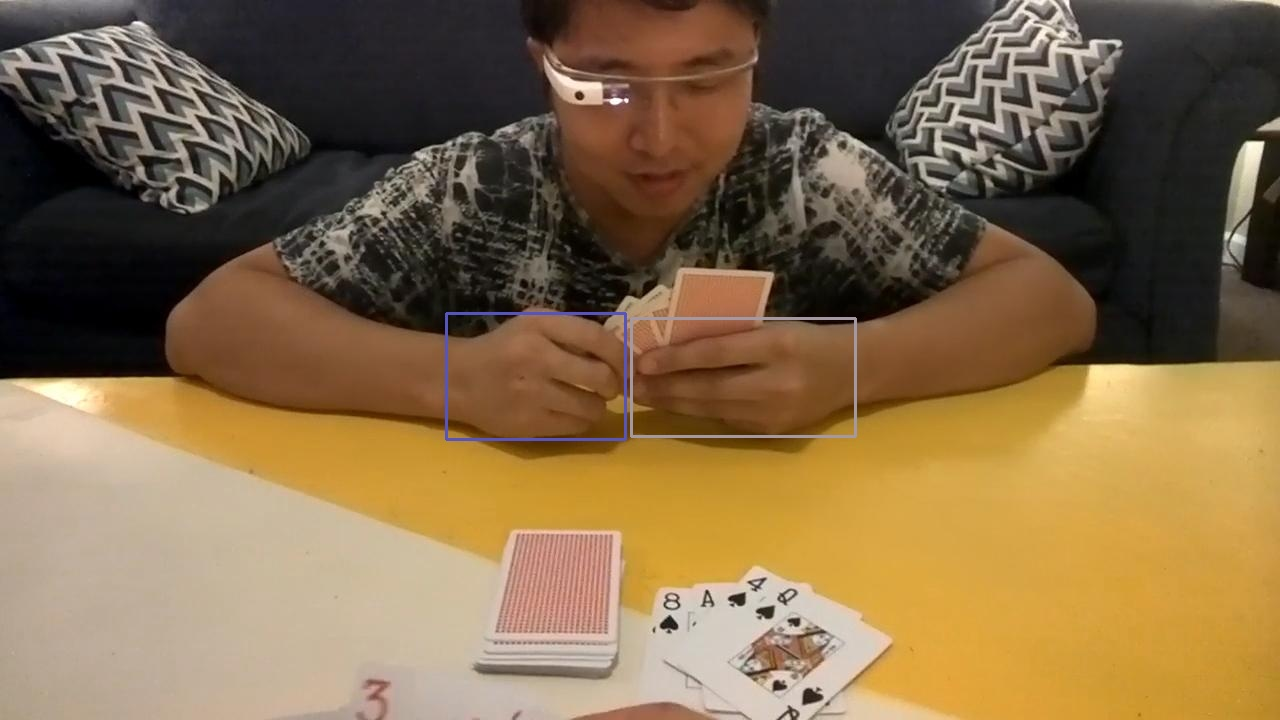
\includegraphics[width=\textwidth]{images/handDetection/01.jpg}
        \caption{01.jpg - Score = 0.996582}
        
    \end{subfigure}
    \hfill
    \begin{subfigure}[b]{0.3\textwidth}
        \centering
        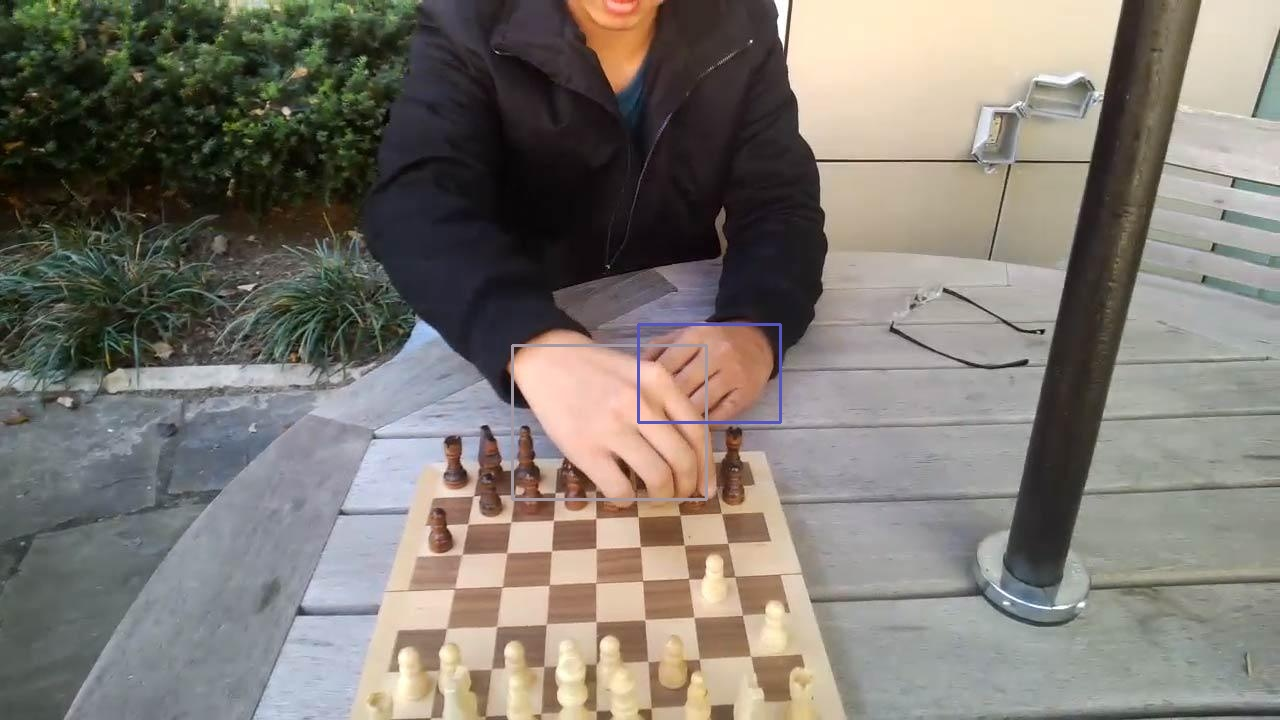
\includegraphics[width=\textwidth]{images/handDetection/02.jpg}
        \caption{02.jpg - Score = 0.949414}
       
    \end{subfigure}
    \hfill
    \begin{subfigure}[b]{0.3\textwidth}
        \centering
        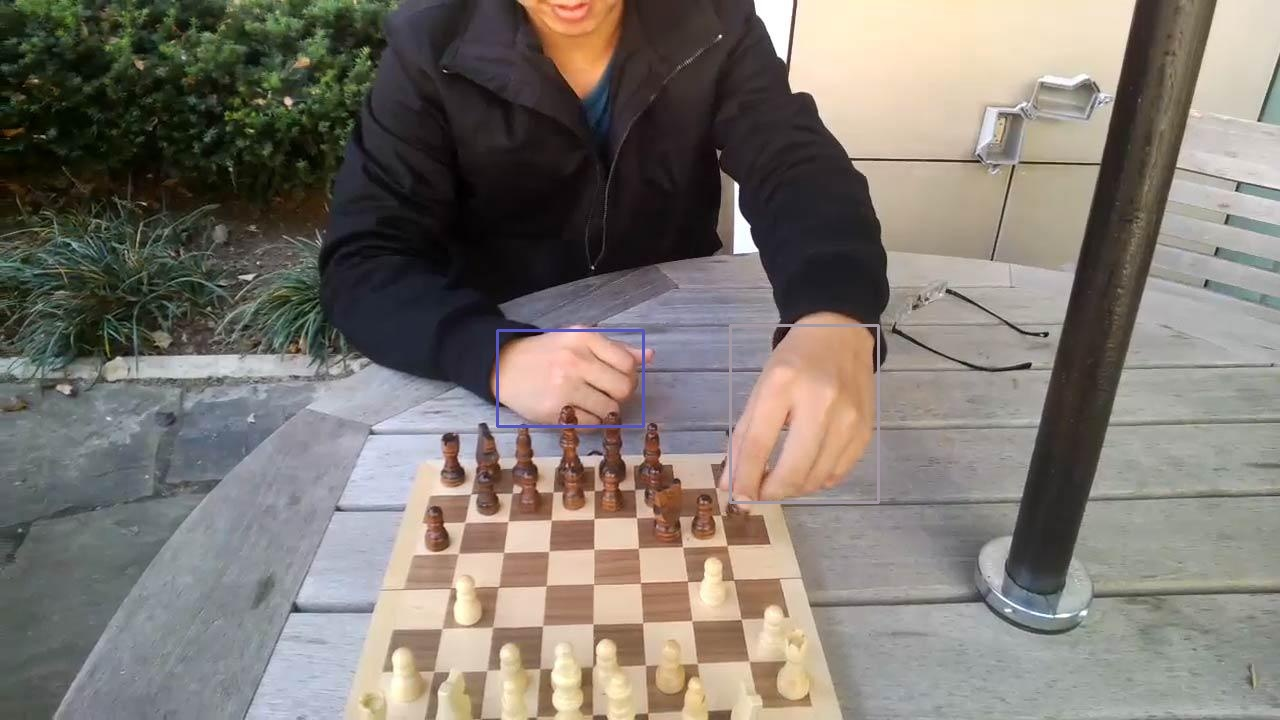
\includegraphics[width=\textwidth]{images/handDetection/03.jpg}
        \caption{03.jpg - Score = 0.995508}
       
    \end{subfigure}

    \begin{subfigure}[b]{0.3 \textwidth}
        \centering
        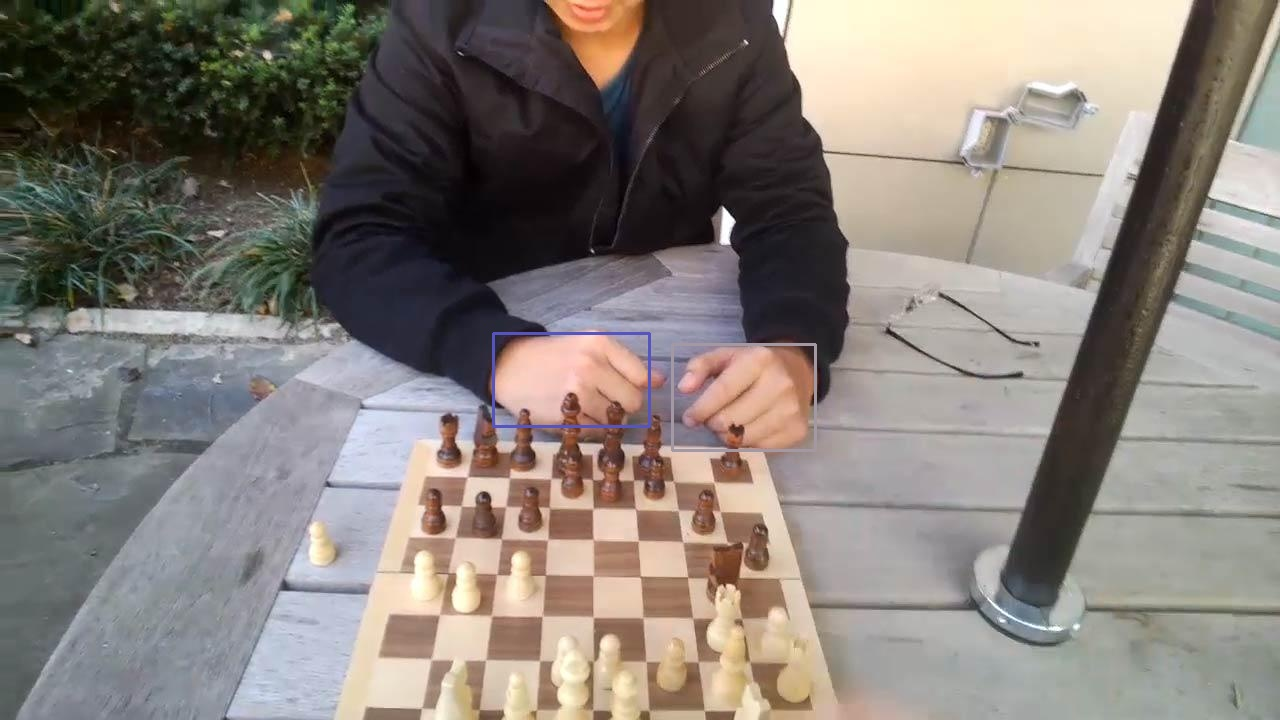
\includegraphics[width=\textwidth]{images/handDetection/04.jpg}
        \caption{04.jpg - Score = 0.994824}
       
    \end{subfigure}
    \hfill
    \begin{subfigure}[b]{0.3\textwidth}
        \centering
        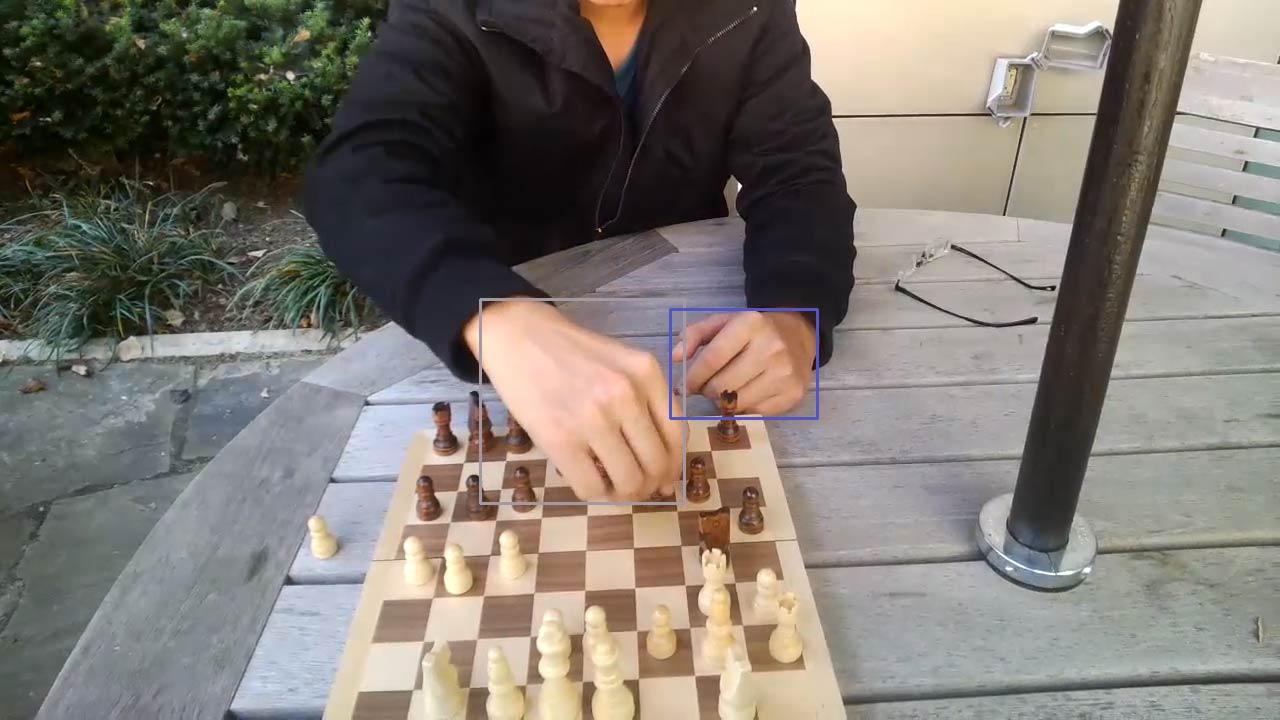
\includegraphics[width=\textwidth]{images/handDetection/05.jpg}
        \caption{05.jpg - Score = 0.932324}
        
    \end{subfigure}
    \hfill
    \begin{subfigure}[b]{0.3\textwidth}
        \centering
        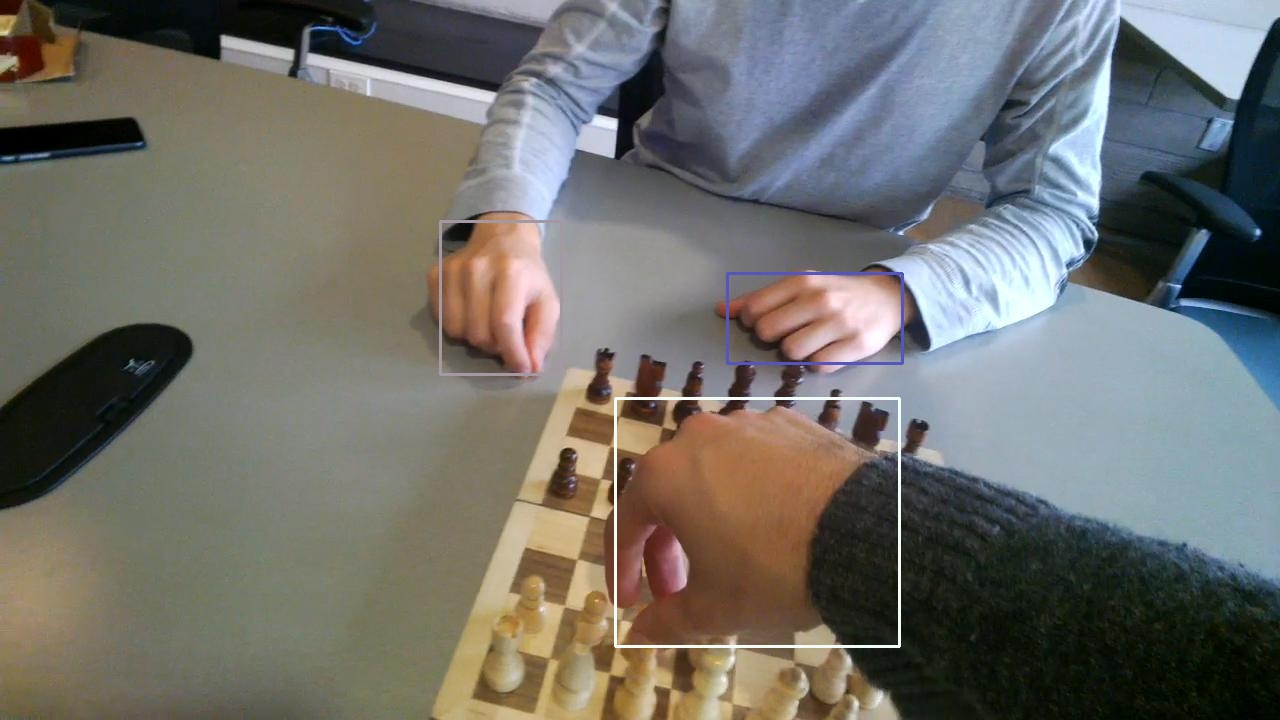
\includegraphics[width=\textwidth]{images/handDetection/06.jpg}
        \caption{06.jpg - Score = 0.922852}
        
    \end{subfigure}
       
    \begin{subfigure}[b]{0.3 \textwidth}
        \centering
        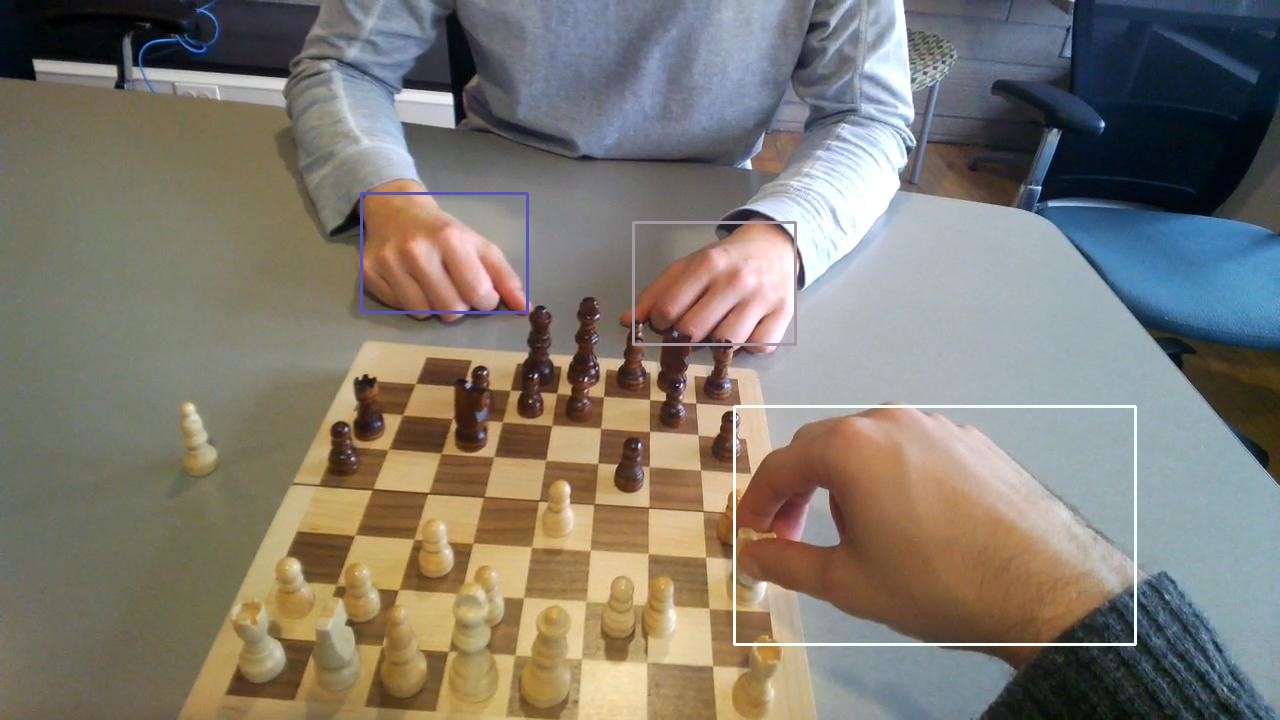
\includegraphics[width=\textwidth]{images/handDetection/07.jpg}
        \caption{07.jpg - Score = 0.876497}
        
    \end{subfigure}
    \hfill
    \begin{subfigure}[b]{0.3\textwidth}
        \centering
        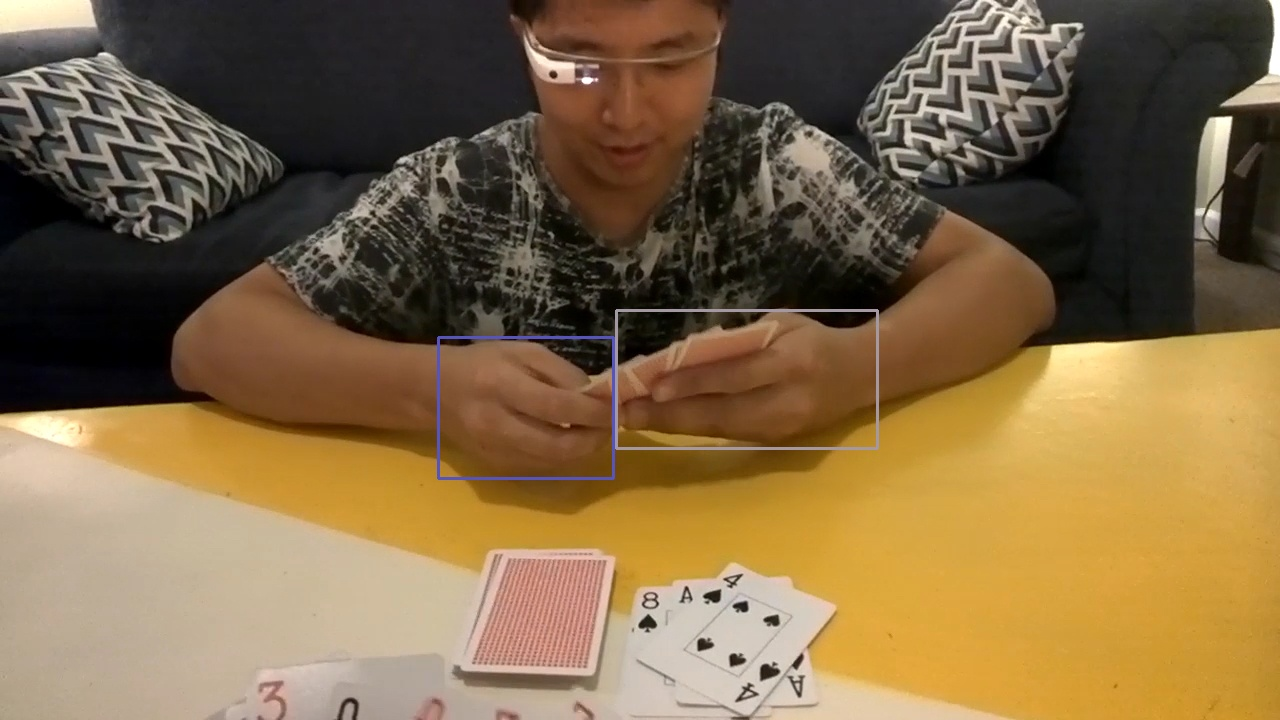
\includegraphics[width=\textwidth]{images/handDetection/08.jpg}
        \caption{08.jpg - Score = 0.994336}
       
    \end{subfigure}
    \hfill
    \begin{subfigure}[b]{0.3\textwidth}
        \centering
        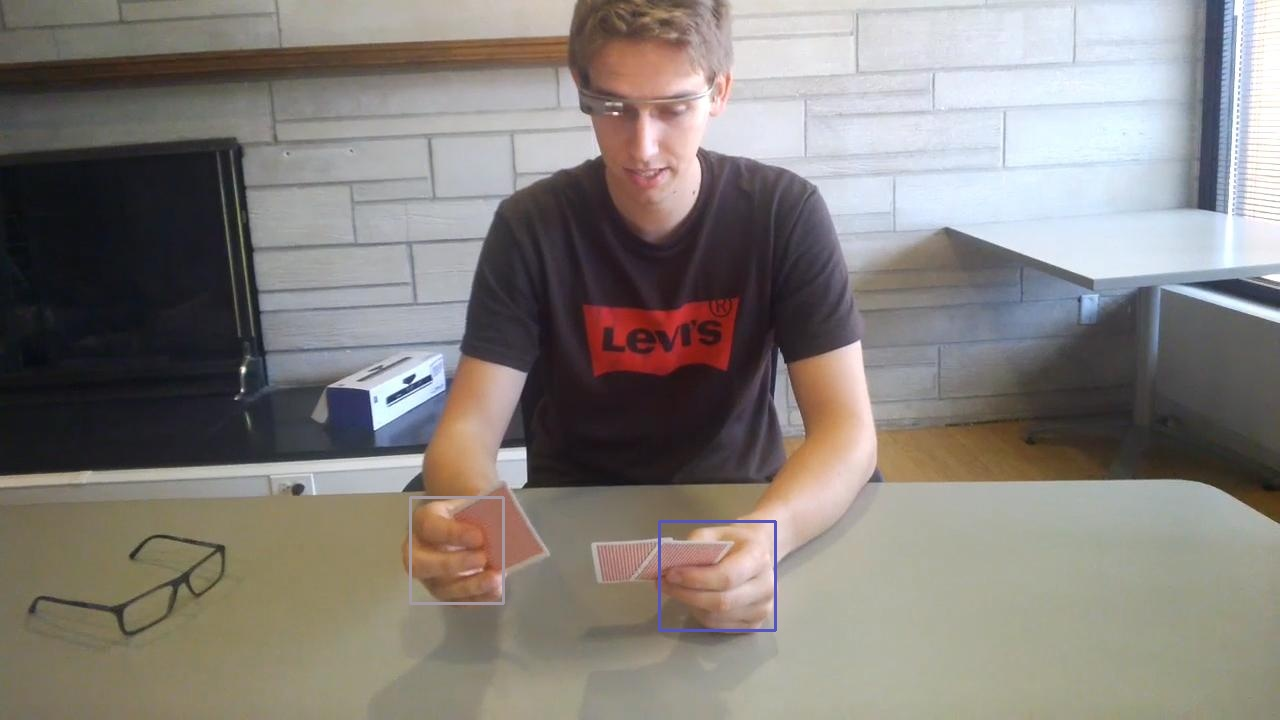
\includegraphics[width=\textwidth]{images/handDetection/09.jpg}
        \caption{09.jpg - Score = 0.938281}
        
    \end{subfigure}
       
    \begin{subfigure}[b]{0.3 \textwidth}
        \centering
        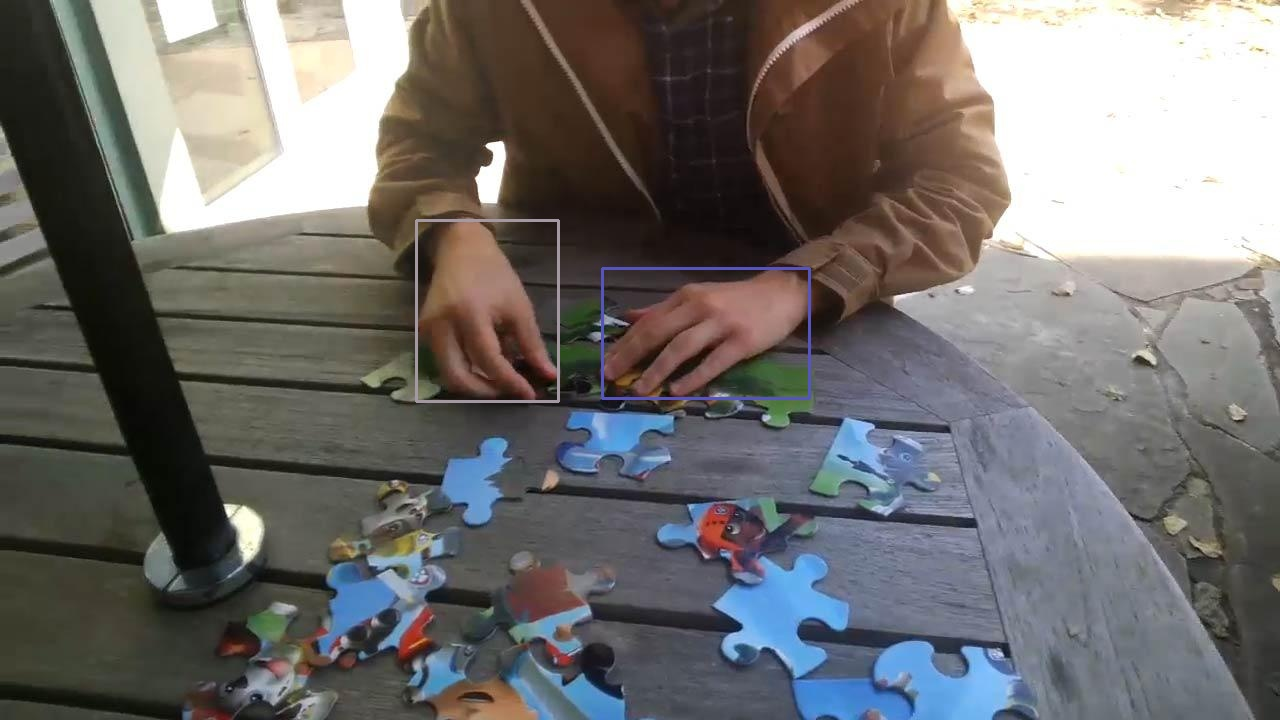
\includegraphics[width=\textwidth]{images/handDetection/10.jpg}
        \caption{10.jpg - Score = 0.931445}
        
    \end{subfigure}
    \hfill
    \begin{subfigure}[b]{0.3\textwidth}
        \centering
        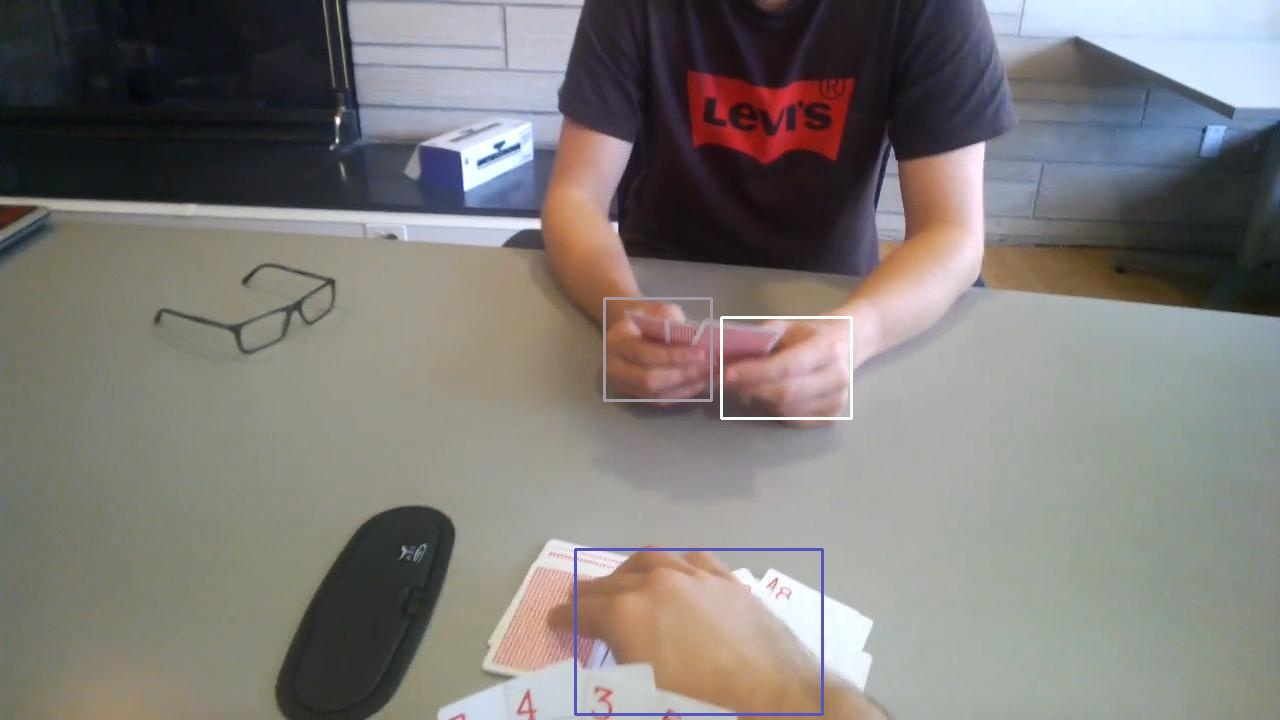
\includegraphics[width=\textwidth]{images/handDetection/11.jpg}
        \caption{11.jpg - Score = 0.918620}
        
    \end{subfigure}
    \hfill
    \begin{subfigure}[b]{0.3\textwidth}
        \centering
        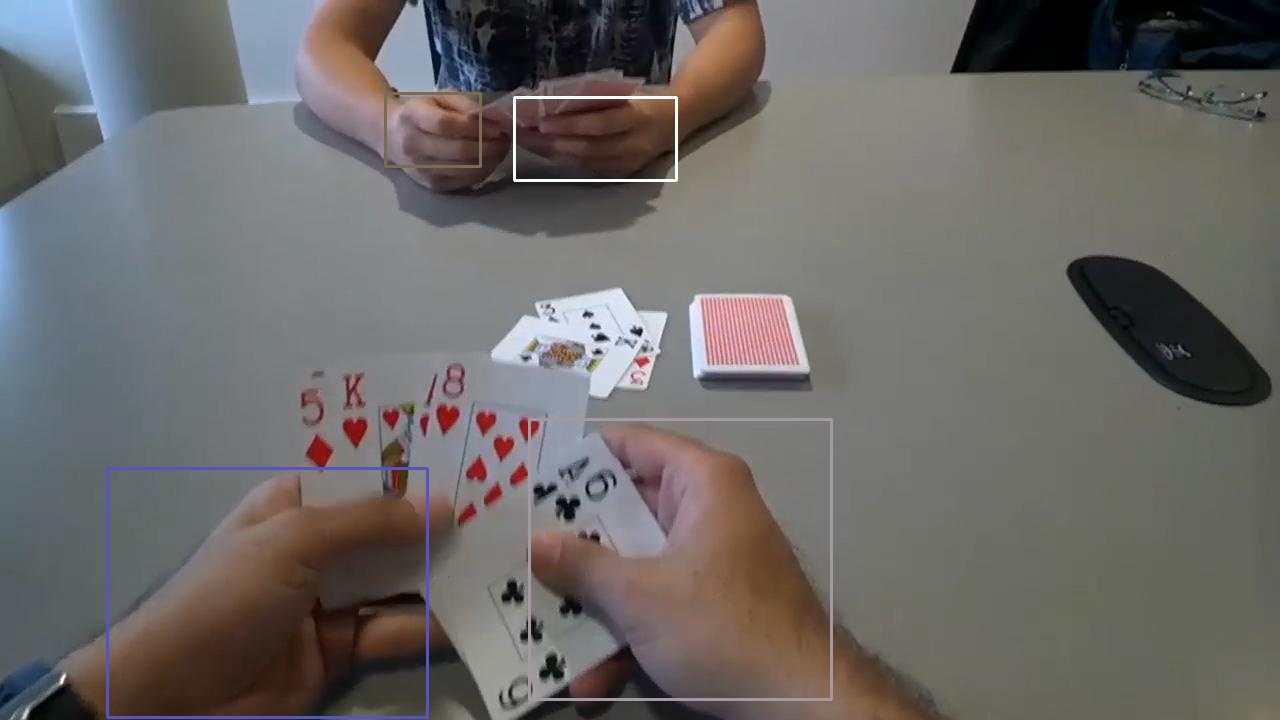
\includegraphics[width=\textwidth]{images/handDetection/12.jpg}
        \caption{12.jpg - Score = 0.941895}
        
    \end{subfigure}
    \caption{Detection on dataset samples 01-12}
       
\end{figure}



\begin{figure}[!h]
    \centering
    \begin{subfigure}[b]{0.3 \textwidth}
        \centering
        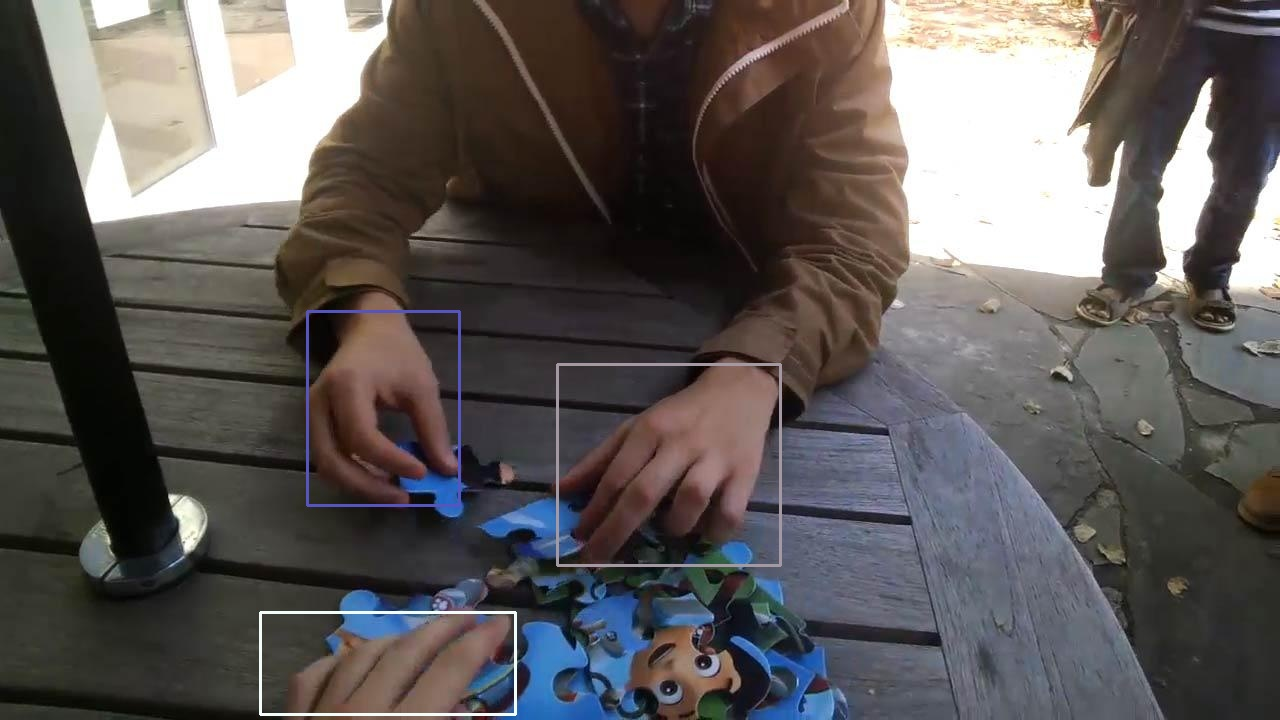
\includegraphics[width=\textwidth]{images/handDetection/13.jpg}
        \caption{13.jpg - Score = 0.899609}
        
    \end{subfigure}
    \hfill
    \begin{subfigure}[b]{0.3\textwidth}
        \centering
        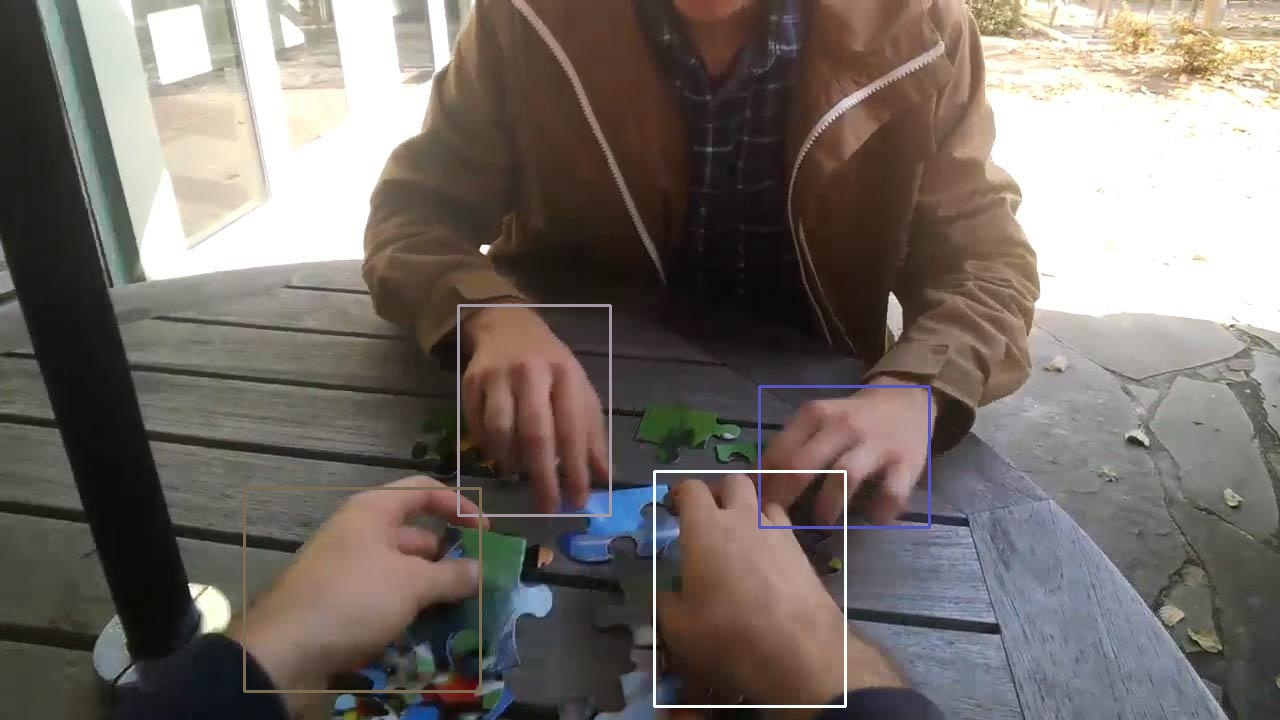
\includegraphics[width=\textwidth]{images/handDetection/14.jpg}
        \caption{14.jpg - Score = 0.925391}
        
    \end{subfigure}
    \hfill
    \begin{subfigure}[b]{0.3\textwidth}
        \centering
        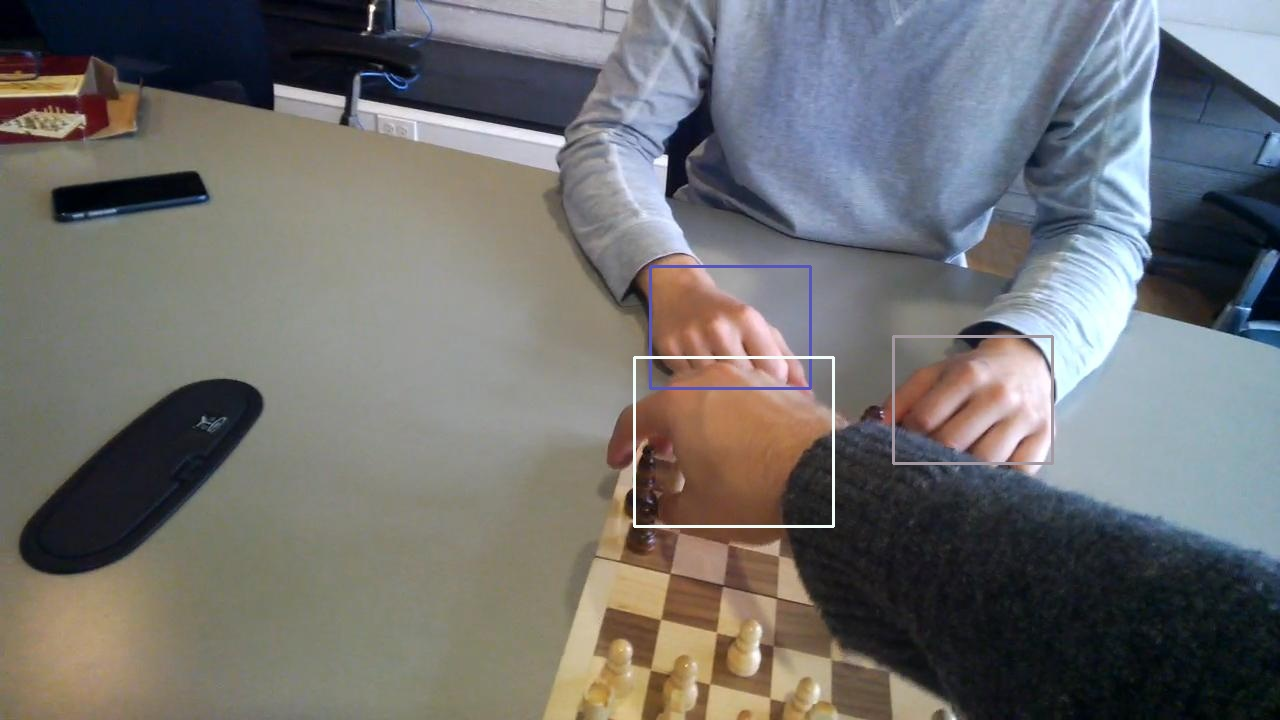
\includegraphics[width=\textwidth]{images/handDetection/15.jpg}
        \caption{15.jpg - Score = 0.939063}
       
    \end{subfigure}

    \begin{subfigure}[b]{0.3 \textwidth}
        \centering
        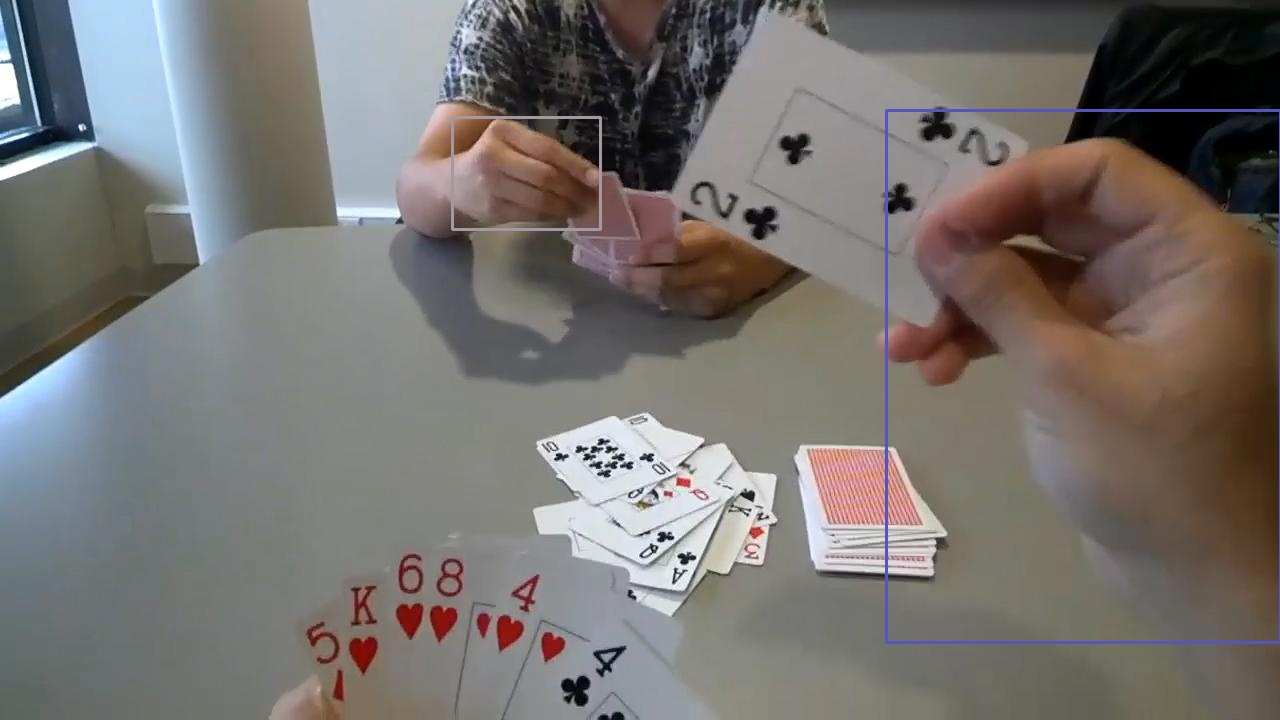
\includegraphics[width=\textwidth]{images/handDetection/16.jpg}
        \caption{16.jpg - Score = 0.898242}
        
    \end{subfigure}
    \hfill
    \begin{subfigure}[b]{0.3\textwidth}
        \centering
        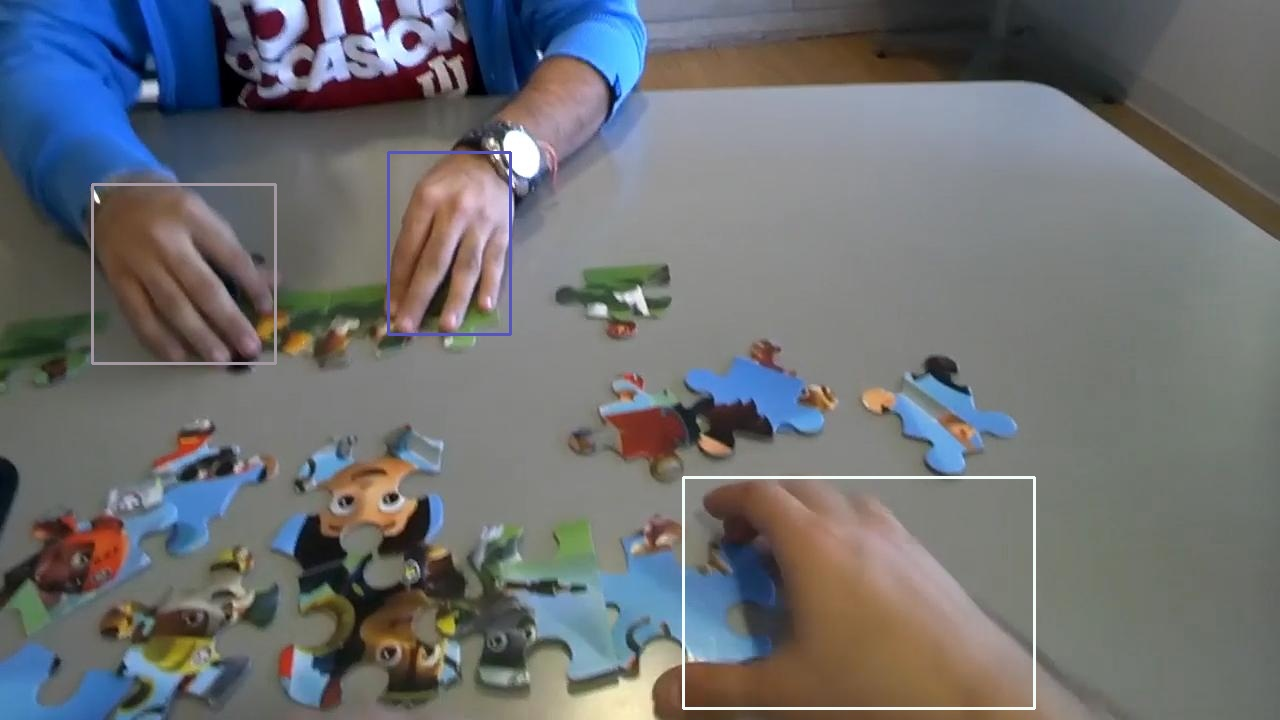
\includegraphics[width=\textwidth]{images/handDetection/17.jpg}
        \caption{17.jpg - Score = 0.851823}
        
    \end{subfigure}
    \hfill
    \begin{subfigure}[b]{0.3\textwidth}
        \centering
        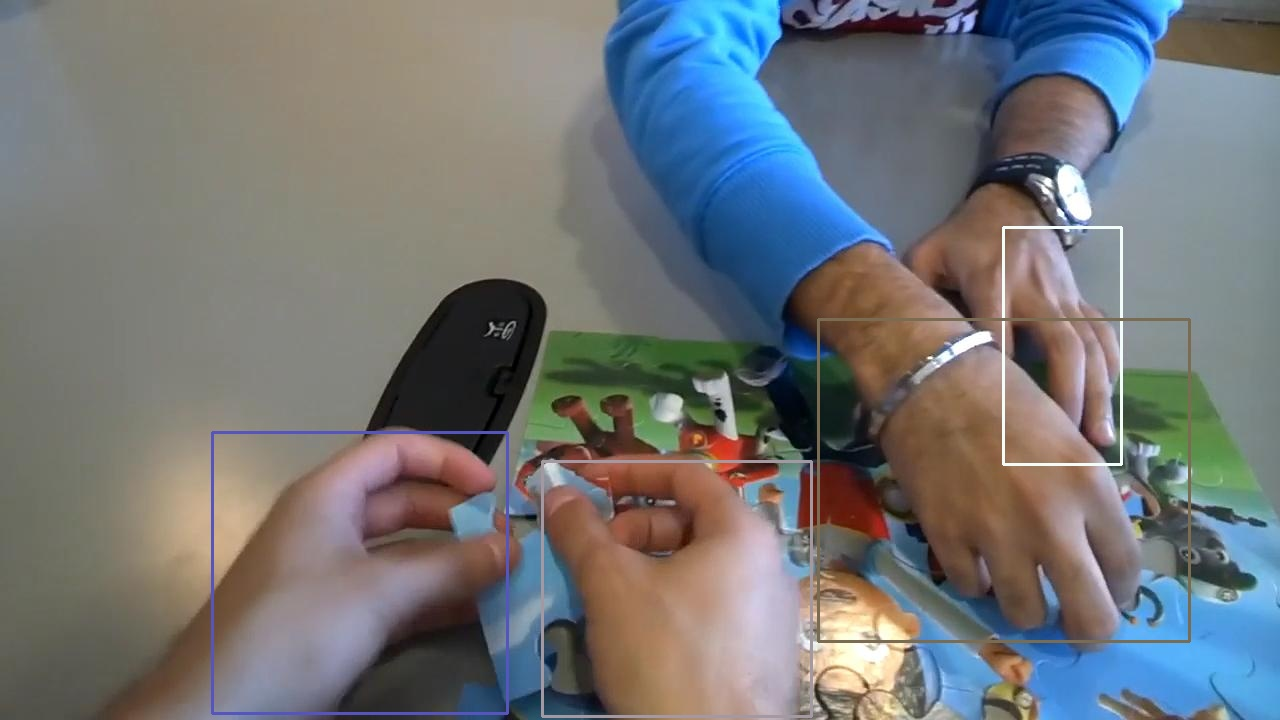
\includegraphics[width=\textwidth]{images/handDetection/18.jpg}
        \caption{18.jpg - Score = 0.931738}
        
    \end{subfigure}
       
    \begin{subfigure}[b]{0.3 \textwidth}
        \centering
        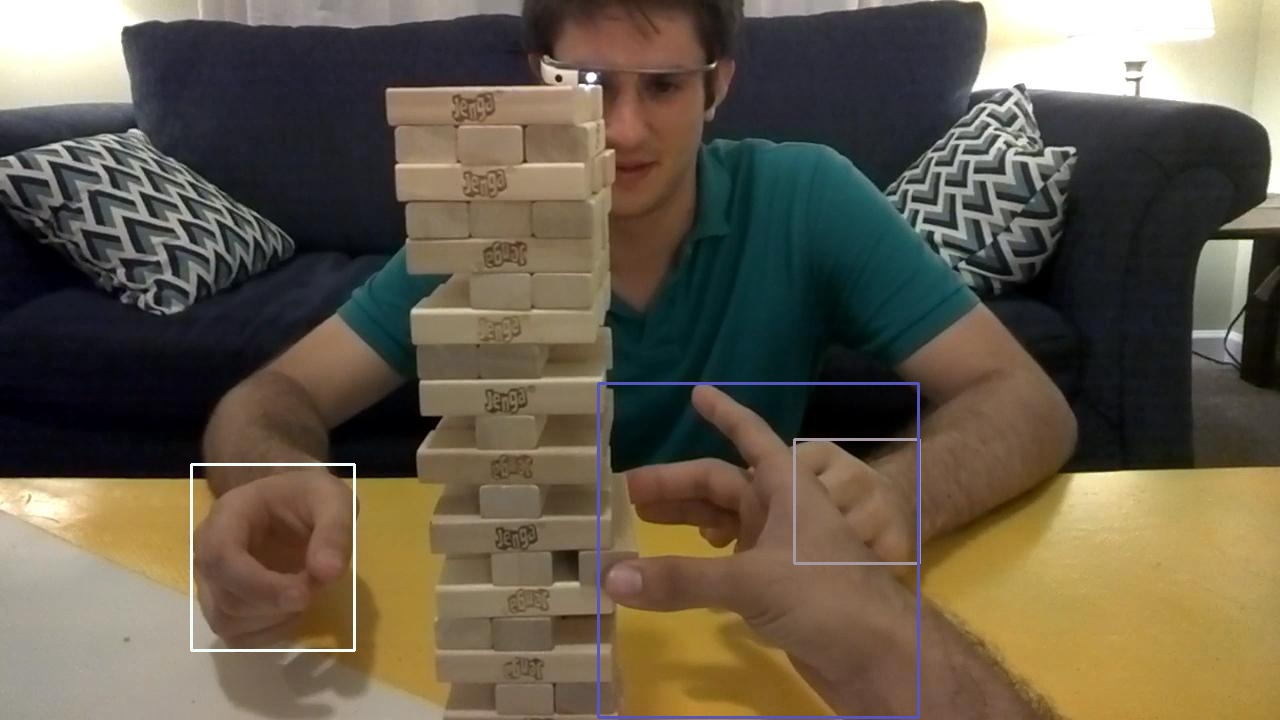
\includegraphics[width=\textwidth]{images/handDetection/19.jpg}
        \caption{19.jpg - Score = 0.918034}
        
    \end{subfigure}
    \hfill
    \begin{subfigure}[b]{0.3\textwidth}
        \centering
        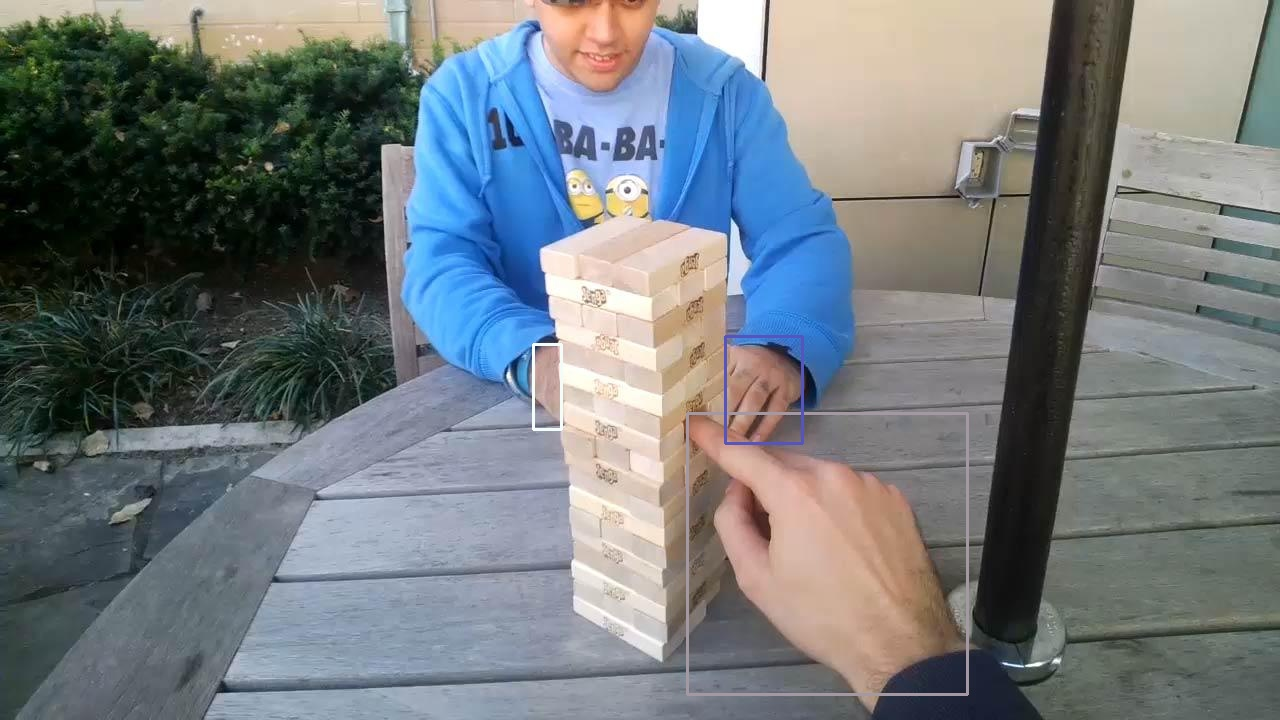
\includegraphics[width=\textwidth]{images/handDetection/20.jpg}
        \caption{20.jpg - Score = 0.994336}
        
    \end{subfigure}
    \hfill
    \begin{subfigure}[b]{0.3\textwidth}
        \centering
        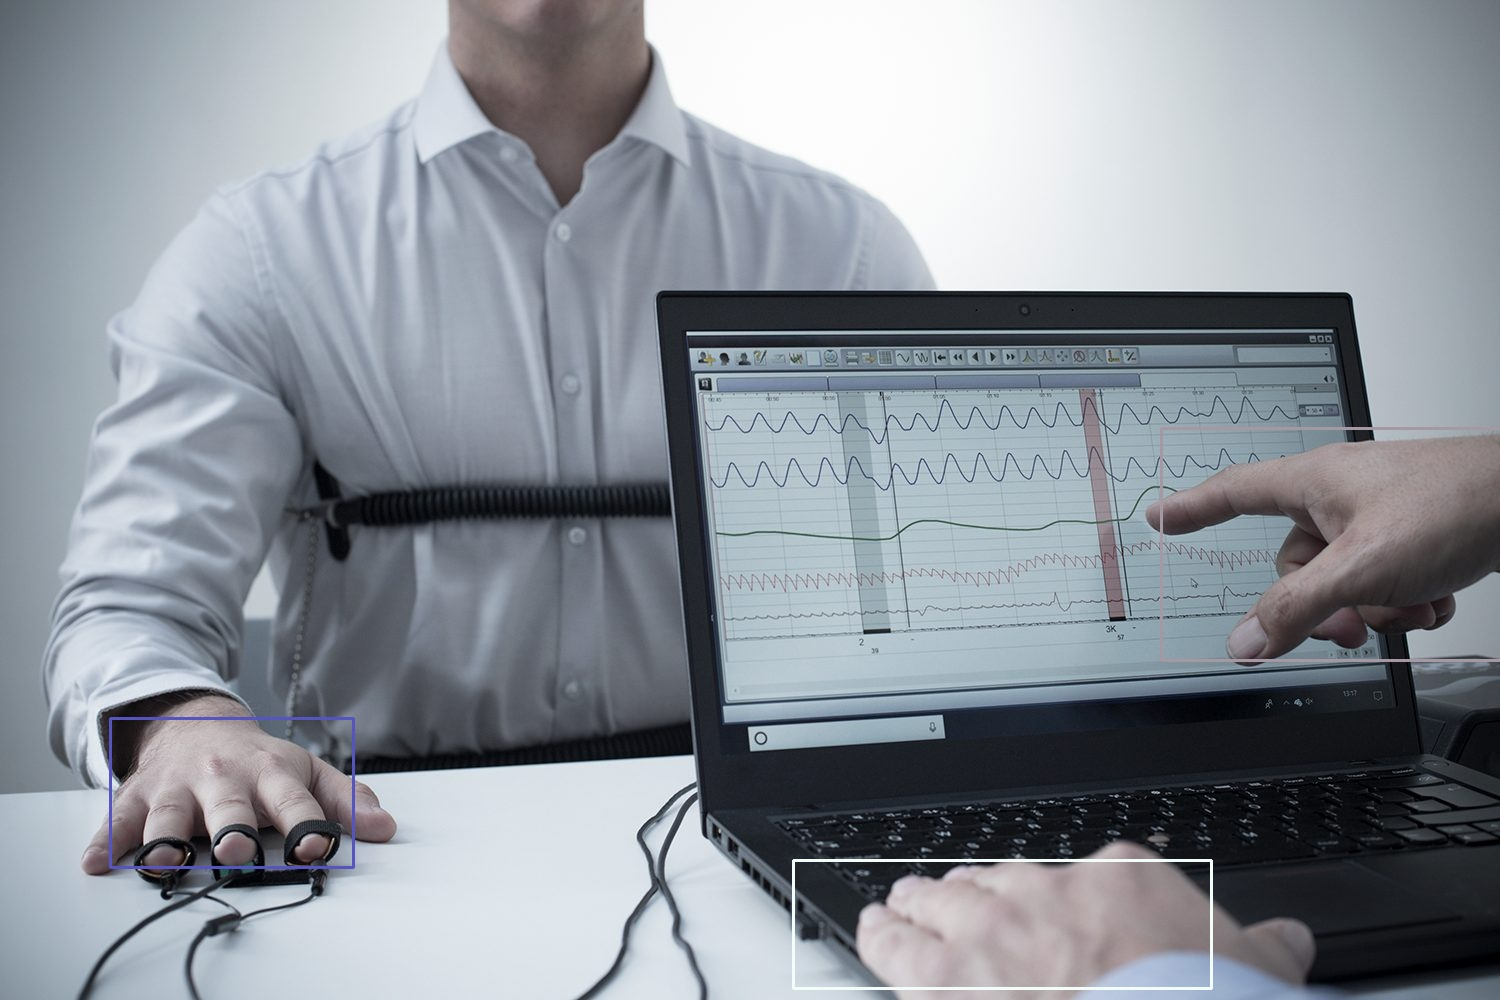
\includegraphics[width=\textwidth]{images/handDetection/test.jpg}
        \caption{Random image}
        
    \end{subfigure}
    \caption{Detection on dataset samples 13-20}
       
\end{figure}

\clearpage

Here are the numerical results of the bounding boxes (x,y,width,height) of the hand detected in the images.
% Please add the following required packages to your document preamble:
% \usepackage[table,xcdraw]{xcolor}
% If you use beamer only pass "xcolor=table" option, i.e. \documentclass[xcolor=table]{beamer}
\begin{table}[h!]
    \centering
    \begin{tabular}{ccc}
    \rowcolor[HTML]{BCBCBC} 
    \multicolumn{1}{l}{\cellcolor[HTML]{BCBCBC}{\color[HTML]{000000} \textbf{Image}}} & \multicolumn{1}{l}{\cellcolor[HTML]{BCBCBC}{\color[HTML]{000000} \textbf{Score}}} & \multicolumn{1}{l}{\cellcolor[HTML]{BCBCBC}\textbf{Box Values}}                                                                     \\ \hline
    \multicolumn{1}{|c|}{01.jpg}                                                      & \multicolumn{1}{c|}{0.996582}                                                     & \multicolumn{1}{c|}{\begin{tabular}[c]{@{}c@{}}631,318,224,118\\ 446,313,179,126\end{tabular}}                                      \\ \hline
    \multicolumn{1}{|c|}{02.jpg}                                                      & \multicolumn{1}{c|}{0.949414}                                                     & \multicolumn{1}{c|}{\begin{tabular}[c]{@{}c@{}}512,345,194,154\\ 638,324,142,98\end{tabular}}                                       \\ \hline
    \multicolumn{1}{|c|}{03.jpg}                                                      & \multicolumn{1}{c|}{0.995508}                                                     & \multicolumn{1}{c|}{\begin{tabular}[c]{@{}c@{}}730,325,148,177\\ 497,330,146,96\end{tabular}}                                       \\ \hline
    \multicolumn{1}{|c|}{04.jpg}                                                      & \multicolumn{1}{c|}{0.994824}                                                     & \multicolumn{1}{c|}{\begin{tabular}[c]{@{}c@{}}672,344,143,106\\ 493,333,156,93\end{tabular}}                                       \\ \hline
    \multicolumn{1}{|c|}{05.jpg}                                                      & \multicolumn{1}{c|}{0.932324}                                                     & \multicolumn{1}{c|}{\begin{tabular}[c]{@{}c@{}}480,299,204,204\\ 670,309,147,109\end{tabular}}                                      \\ \hline
    \multicolumn{1}{|c|}{06.jpg}                                                      & \multicolumn{1}{c|}{0.922852}                                                     & \multicolumn{1}{c|}{\begin{tabular}[c]{@{}c@{}}440,221,121,153\\ 727,273,175,90\\ 615,398,284,248\end{tabular}}                     \\ \hline
    \multicolumn{1}{|c|}{07.jpg}                                                      & \multicolumn{1}{c|}{0.876497}                                                     & \multicolumn{1}{c|}{\begin{tabular}[c]{@{}c@{}}633,222,162,122\\ 361,193,166,119\\ 734,406,401,238\end{tabular}}                    \\ \hline
    \multicolumn{1}{|c|}{08.jpg}                                                      & \multicolumn{1}{c|}{0.994336}                                                     & \multicolumn{1}{c|}{\begin{tabular}[c]{@{}c@{}}616,310,261,138\\ 438,337,175,141\end{tabular}}                                      \\ \hline
    \multicolumn{1}{|c|}{09.jpg}                                                      & \multicolumn{1}{c|}{0.938281}                                                     & \multicolumn{1}{c|}{\begin{tabular}[c]{@{}c@{}}410,497,93,106\\ 659,521,116,109\end{tabular}}                                       \\ \hline
    \multicolumn{1}{|c|}{10.jpg}                                                      & \multicolumn{1}{c|}{0.931445}                                                     & \multicolumn{1}{c|}{\begin{tabular}[c]{@{}c@{}}416,220,142,181\\ 602,268,207,130\end{tabular}}                                      \\ \hline
    \multicolumn{1}{|c|}{11.jpg}                                                      & \multicolumn{1}{c|}{0.918620}                                                     & \multicolumn{1}{c|}{\begin{tabular}[c]{@{}c@{}}604,298,107,102\\ 575,549,247,165\\ 721,317,130,101\end{tabular}}                    \\ \hline
    \multicolumn{1}{|c|}{12.jpg}                                                      & \multicolumn{1}{c|}{0.941895}                                                     & \multicolumn{1}{c|}{\begin{tabular}[c]{@{}c@{}}529,419,302,280\\ 107,468,320,249\\ 514,97,162,83\\ 385,93,95,73\end{tabular}}       \\ \hline
    \multicolumn{1}{|c|}{13.jpg}                                                      & \multicolumn{1}{c|}{0.899609}                                                     & \multicolumn{1}{c|}{\begin{tabular}[c]{@{}c@{}}557,364,223,201\\ 307,311,152,194\\ 260,612,255,102\end{tabular}}                    \\ \hline
    \end{tabular}
    \end{table}

    % Please add the following required packages to your document preamble:
    % \usepackage[table,xcdraw]{xcolor}
    % If you use beamer only pass "xcolor=table" option, i.e. \documentclass[xcolor=table]{beamer}
    \begin{table}[]
        \centering
        \begin{tabular}{ccc}
        \rowcolor[HTML]{BCBCBC} 
        \multicolumn{1}{l}{\cellcolor[HTML]{BCBCBC}{\color[HTML]{000000} \textbf{Image}}} & \multicolumn{1}{l}{\cellcolor[HTML]{BCBCBC}{\color[HTML]{000000} \textbf{Score}}} & \multicolumn{1}{l}{\cellcolor[HTML]{BCBCBC}\textbf{Box Values}}                                                                     \\ \hline
        \multicolumn{1}{|c|}{14.jpg}                                                      & \multicolumn{1}{c|}{0.925391}                                                     & \multicolumn{1}{c|}{\begin{tabular}[c]{@{}c@{}}458,305,152,210\\ 759,386,170,141\\ 654,471,191,235\\ 244,488,236,203\end{tabular}}  \\ \hline
        \multicolumn{1}{|c|}{15.jpg}                                                      & \multicolumn{1}{c|}{0.939063}                                                     & \multicolumn{1}{c|}{\begin{tabular}[c]{@{}c@{}}893,336,159,127\\ 650,266,160,122\\ 634,357,199,169\end{tabular}}                    \\ \hline
        \multicolumn{1}{|c|}{16.jpg}                                                      & \multicolumn{1}{c|}{0.898242}                                                     & \multicolumn{1}{c|}{\begin{tabular}[c]{@{}c@{}}452,117,148,112\\ 886,110,394,532\end{tabular}}                                      \\ \hline
        \multicolumn{1}{|c|}{17.jpg}                                                      & \multicolumn{1}{c|}{0.851823}                                                     & \multicolumn{1}{c|}{\begin{tabular}[c]{@{}c@{}}92,184,183,179\\ 388,152,122,182\\ 683,477,351,231\end{tabular}}                     \\ \hline
        \multicolumn{1}{|c|}{18.jpg}                                                      & \multicolumn{1}{c|}{0.931738}                                                     & \multicolumn{1}{c|}{\begin{tabular}[c]{@{}c@{}}542,461,269,255\\ 212,432,295,281\\ 1003,227,118,237\\ 818,319,371,322\end{tabular}} \\ \hline
        \multicolumn{1}{|c|}{19.jpg}                                                      & \multicolumn{1}{c|}{0.918034}                                                     & \multicolumn{1}{c|}{\begin{tabular}[c]{@{}c@{}}794,439,125,124\\ 598,383,320,334\\ 191,464,163,186\end{tabular}}                    \\ \hline
        \multicolumn{1}{|c|}{20.jpg}                                                      & \multicolumn{1}{c|}{0.994336}                                                     & \multicolumn{1}{c|}{\begin{tabular}[c]{@{}c@{}}687,413,280,281\\ 725,336,77,107\\ 533,344,28,85\end{tabular}}                       \\ \hline
        \end{tabular}
        \end{table}

\clearpage

\subsection{Hand segmentation [2 hrs]}
\chapterauthor{Roberto del Ben}

All the test for hand segmentation indicate that the discriminative value that has most impact on pixel accuracy is the color bandwidth.
So I looped the algorithm over all the dataset seeking for the most suitable color bandwidth value.
The value with best pixel accuracy so far is $5$, with a overall pixel accuracy of $0.980497$. Results with this value are shown in the following images and numerically summarized in a table
at the end of the section.

\begin{figure}[!h]
    \centering
    \begin{subfigure}[b]{0.3 \textwidth}
        \centering
        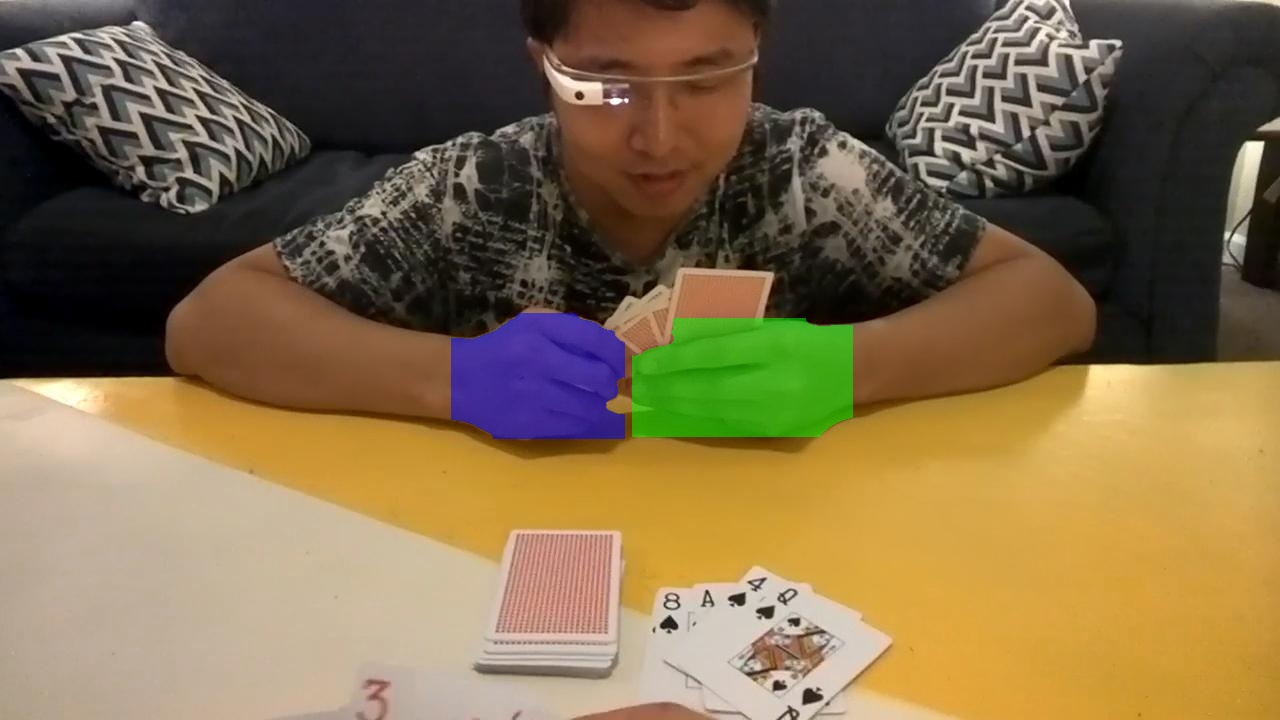
\includegraphics[width=\textwidth]{images/handSegmentation/01.jpg}
        \caption{01.jpg}
        
    \end{subfigure}
    \hfill
    \begin{subfigure}[b]{0.3\textwidth}
        \centering
        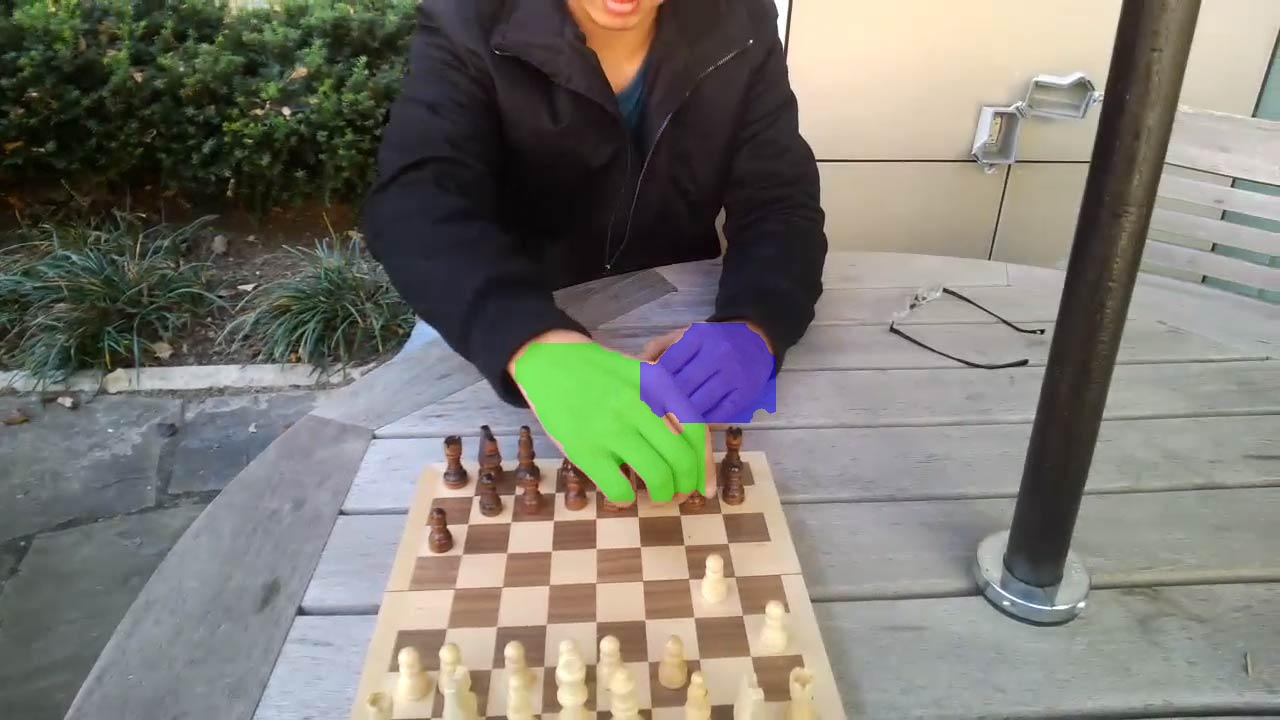
\includegraphics[width=\textwidth]{images/handSegmentation/02.jpg}
        \caption{02.jpg}
       
    \end{subfigure}
    \hfill
    \begin{subfigure}[b]{0.3\textwidth}
        \centering
        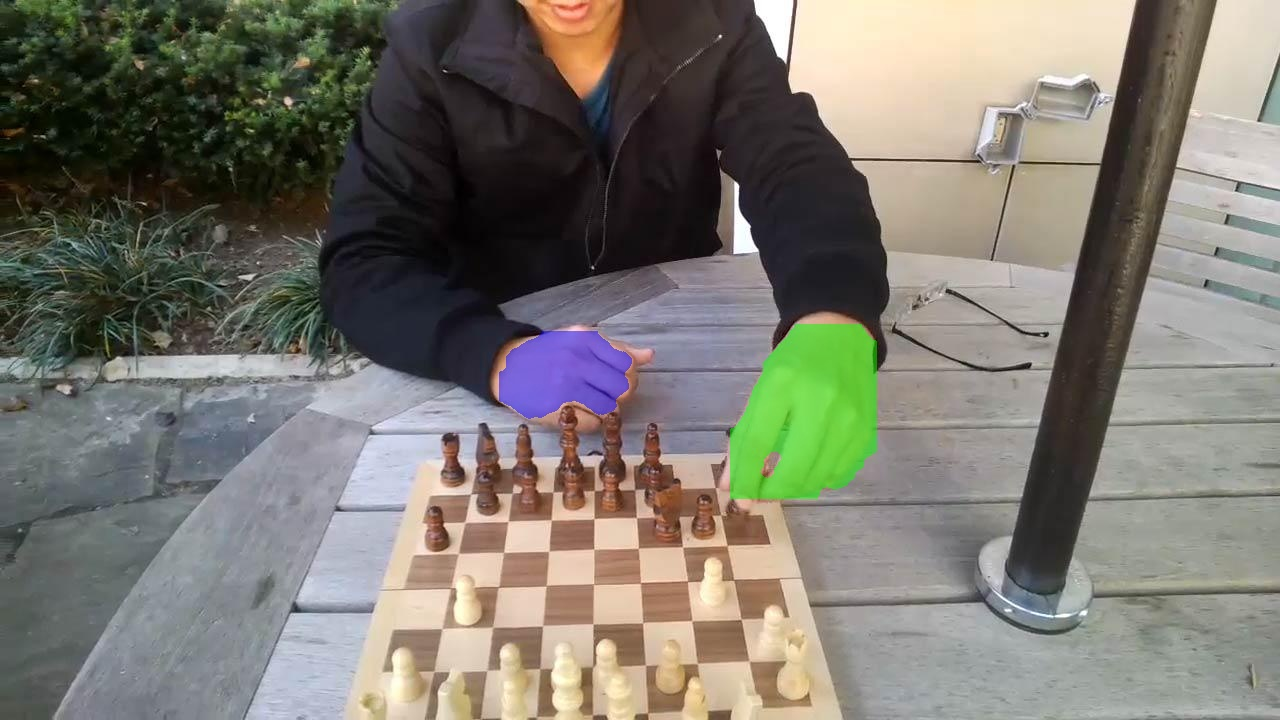
\includegraphics[width=\textwidth]{images/handSegmentation/03.jpg}
        \caption{03.jpg}
       
    \end{subfigure}

    \begin{subfigure}[b]{0.3 \textwidth}
        \centering
        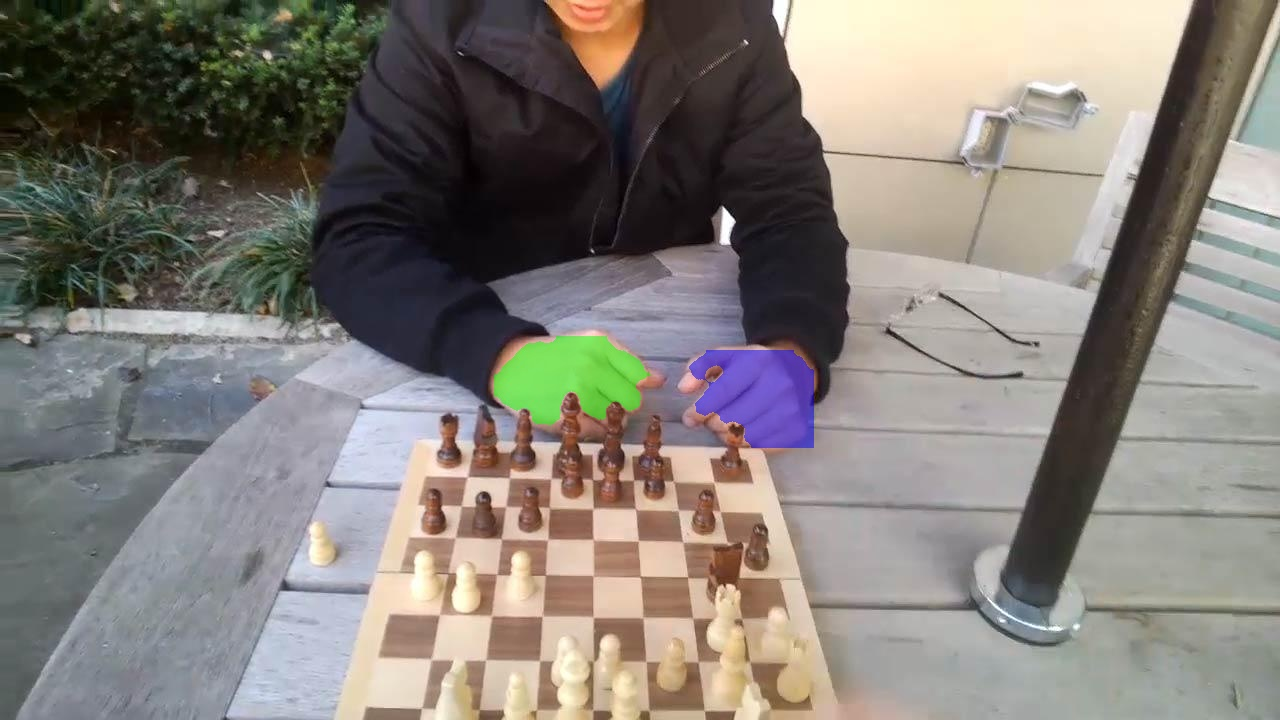
\includegraphics[width=\textwidth]{images/handSegmentation/04.jpg}
        \caption{04.jpg}
       
    \end{subfigure}
    \hfill
    \begin{subfigure}[b]{0.3\textwidth}
        \centering
        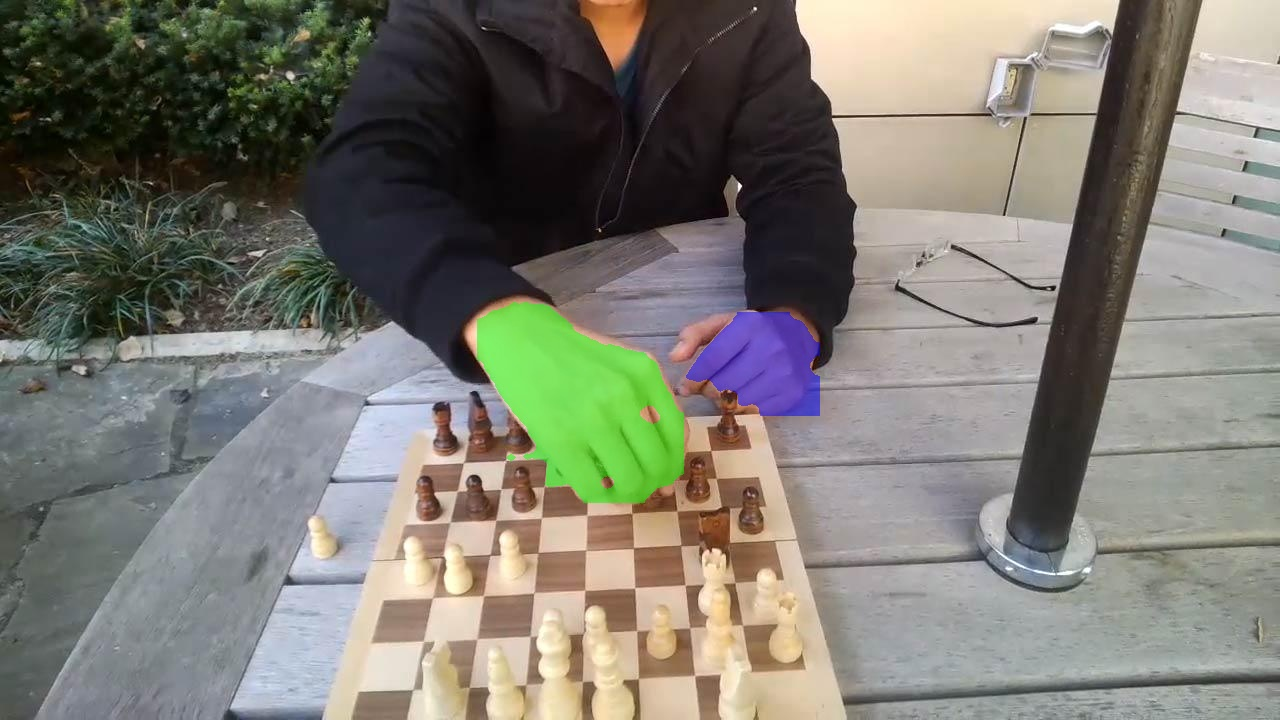
\includegraphics[width=\textwidth]{images/handSegmentation/05.jpg}
        \caption{05.jpg}
        
    \end{subfigure}
    \hfill
    \begin{subfigure}[b]{0.3\textwidth}
        \centering
        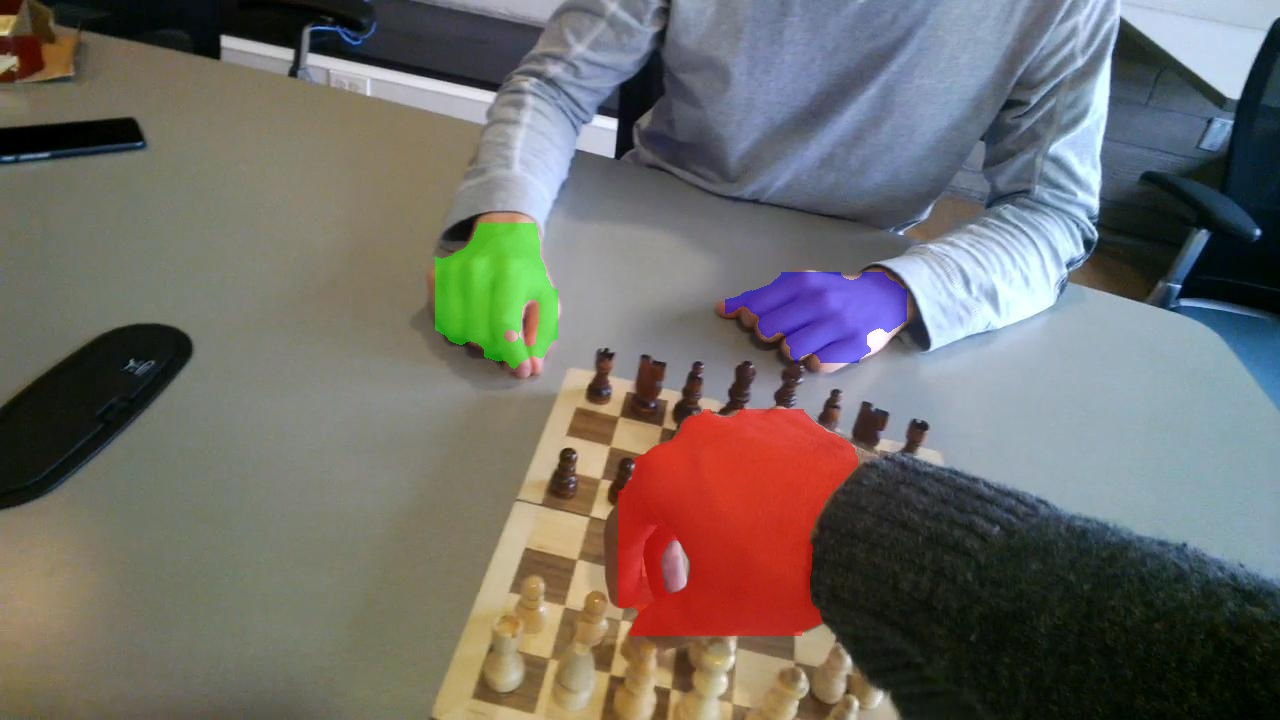
\includegraphics[width=\textwidth]{images/handSegmentation/06.jpg}
        \caption{06.jpg}
        
    \end{subfigure}
       
    \begin{subfigure}[b]{0.3 \textwidth}
        \centering
        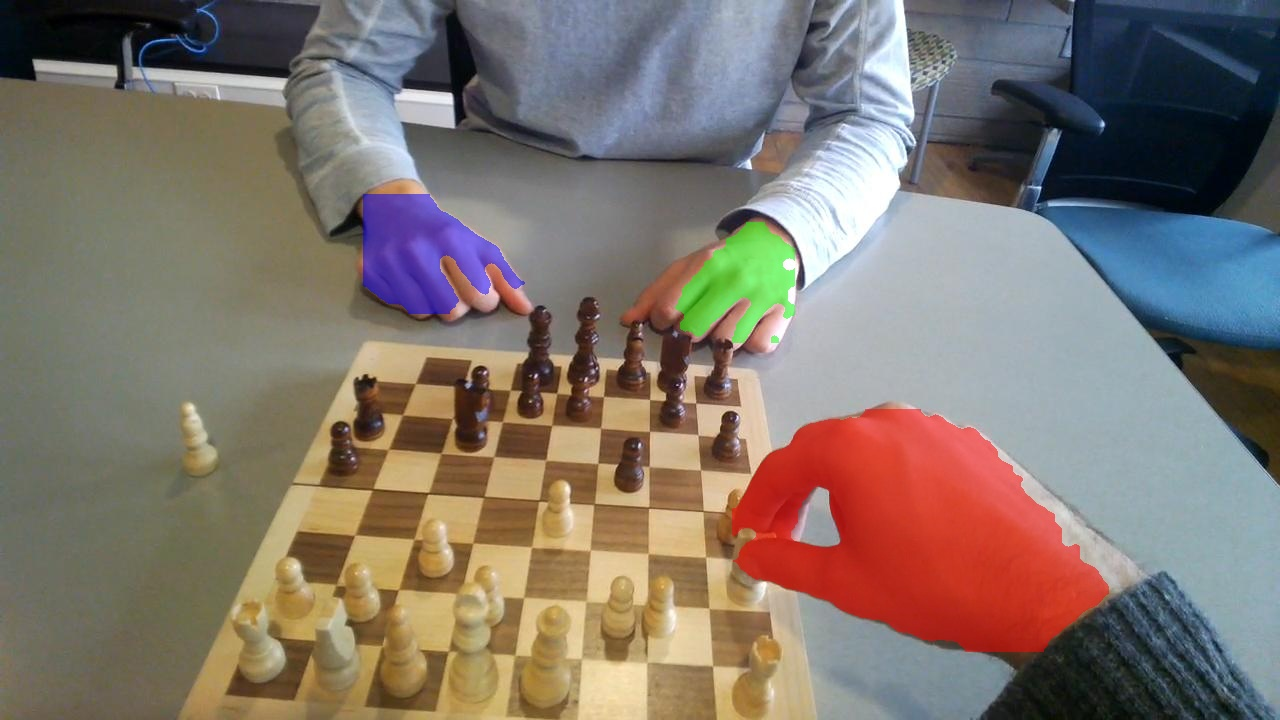
\includegraphics[width=\textwidth]{images/handSegmentation/07.jpg}
        \caption{07.jpg}
        
    \end{subfigure}
    \hfill
    \begin{subfigure}[b]{0.3\textwidth}
        \centering
        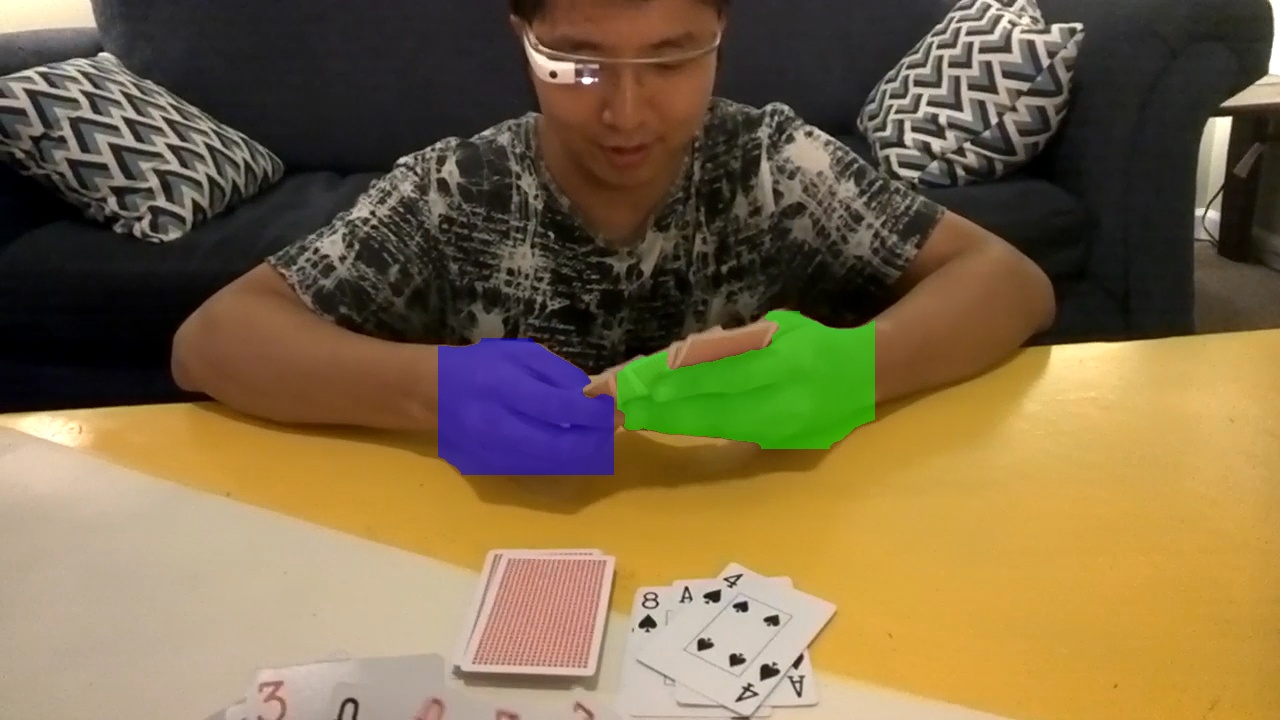
\includegraphics[width=\textwidth]{images/handSegmentation/08.jpg}
        \caption{08.jpg}
       
    \end{subfigure}
    \hfill
    \begin{subfigure}[b]{0.3\textwidth}
        \centering
        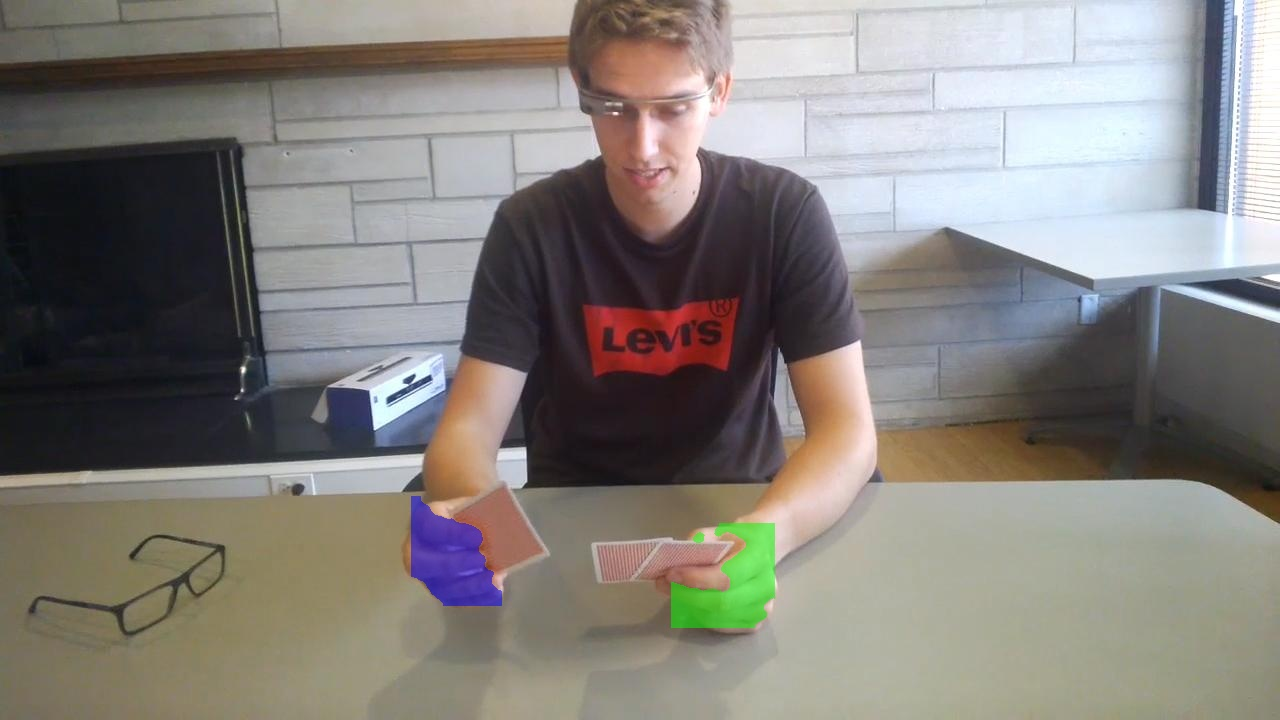
\includegraphics[width=\textwidth]{images/handSegmentation/09.jpg}
        \caption{09.jpg}
        
    \end{subfigure}
       
    \begin{subfigure}[b]{0.3 \textwidth}
        \centering
        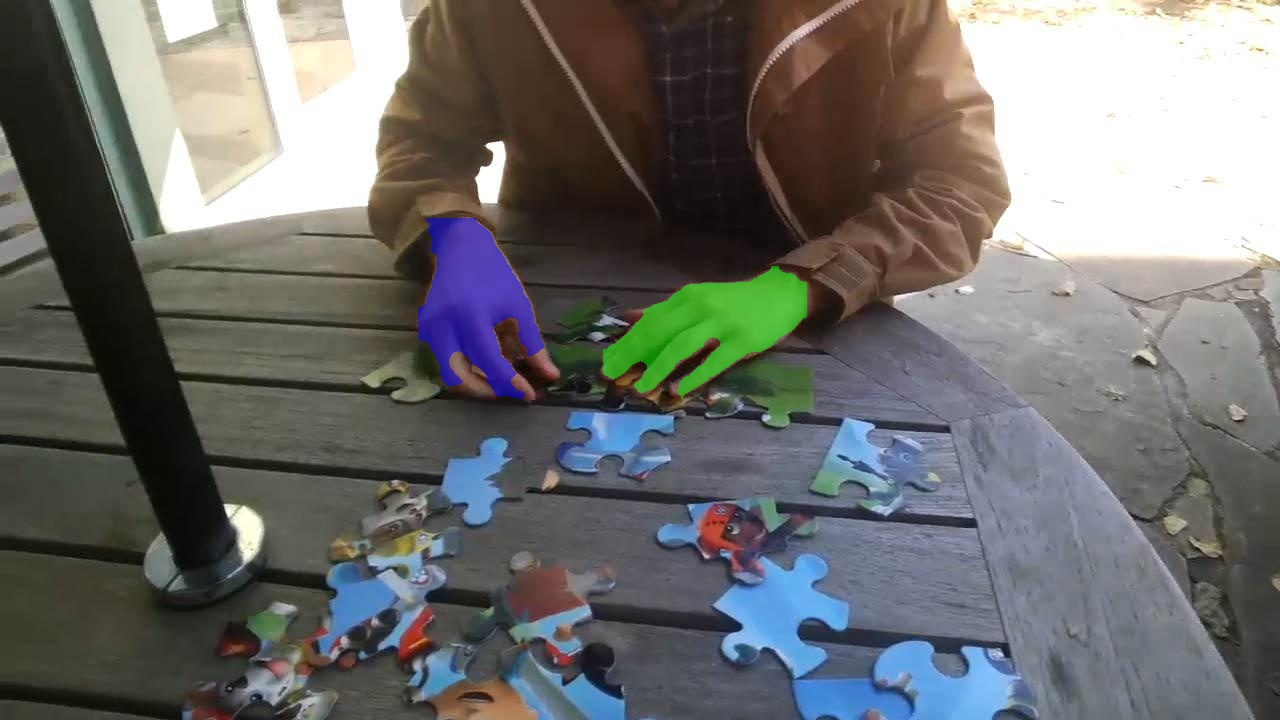
\includegraphics[width=\textwidth]{images/handSegmentation/10.jpg}
        \caption{10.jpg}
        
    \end{subfigure}
    \hfill
    \begin{subfigure}[b]{0.3\textwidth}
        \centering
        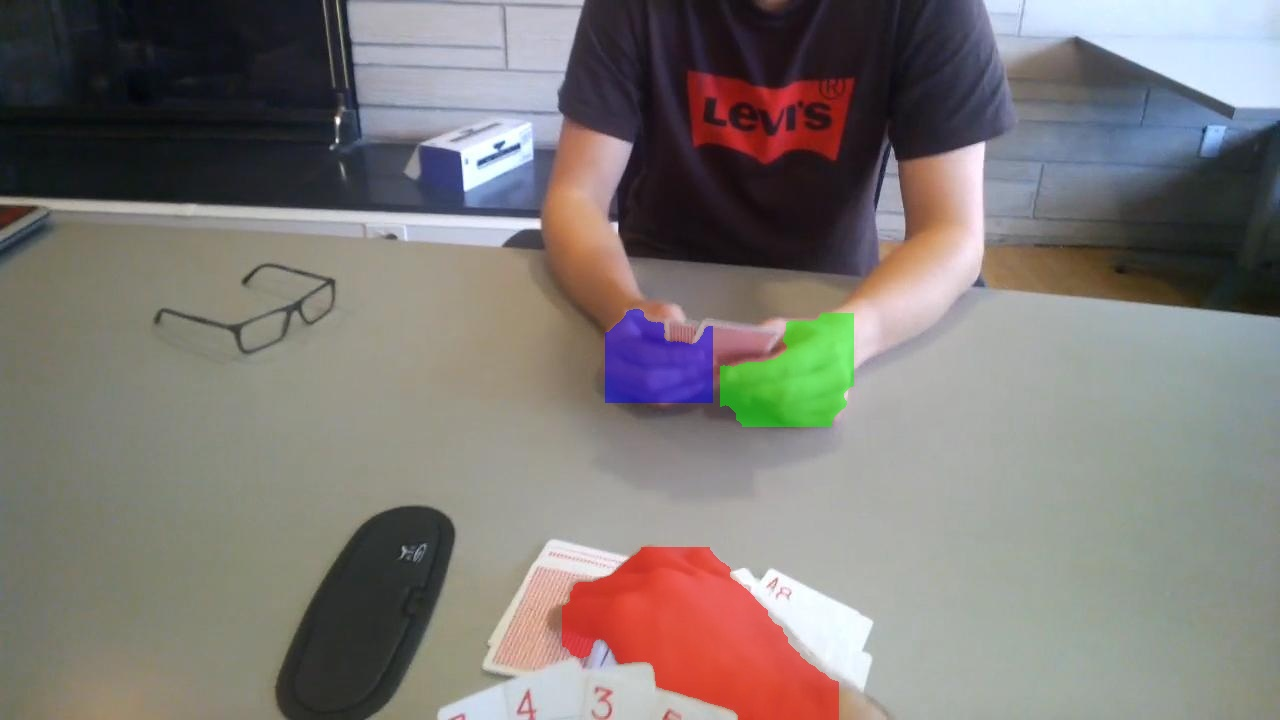
\includegraphics[width=\textwidth]{images/handSegmentation/11.jpg}
        \caption{11.jpg}
        
    \end{subfigure}
    \hfill
    \begin{subfigure}[b]{0.3\textwidth}
        \centering
        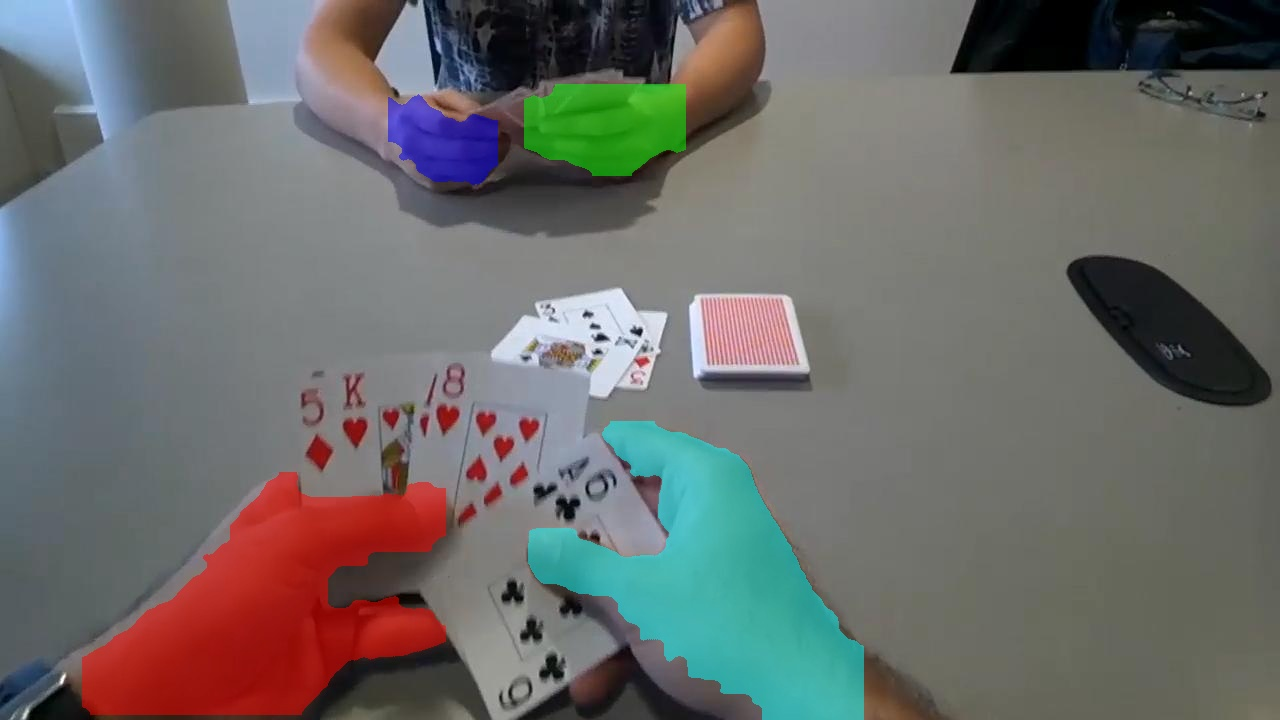
\includegraphics[width=\textwidth]{images/handSegmentation/12.jpg}
        \caption{12.jpg}
        
    \end{subfigure}

        \begin{subfigure}[b]{0.3 \textwidth}
        \centering
        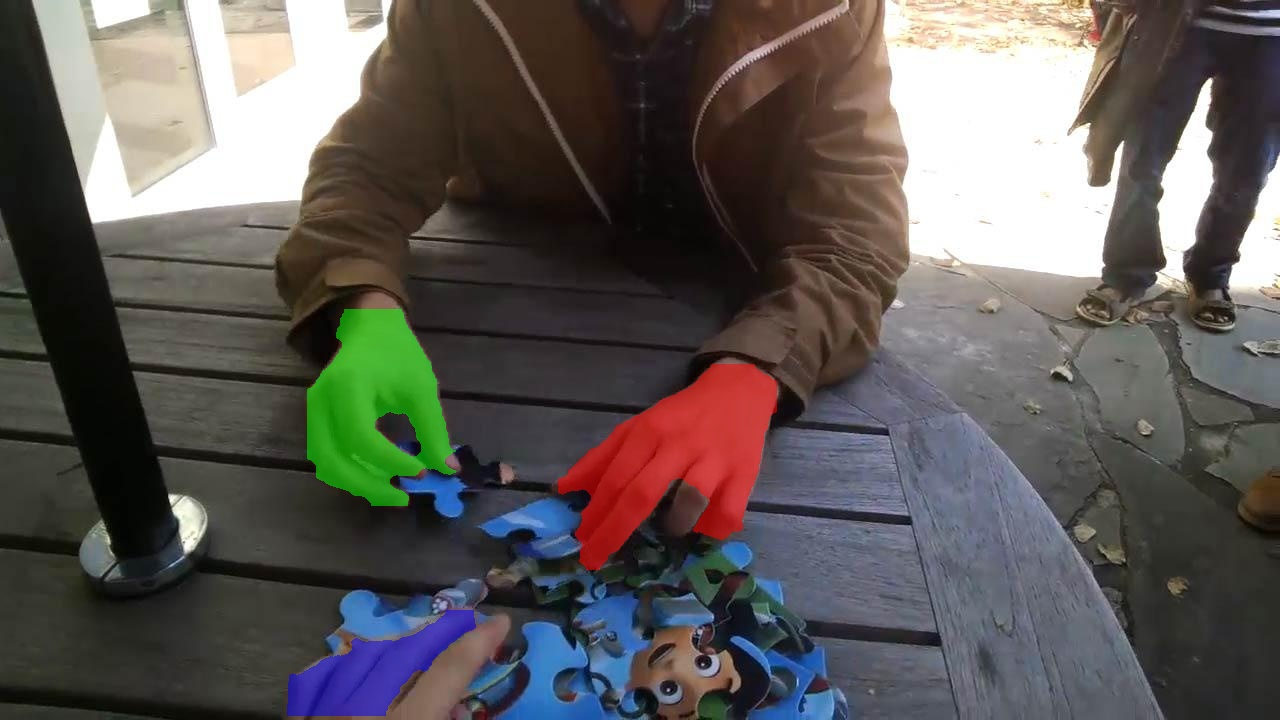
\includegraphics[width=\textwidth]{images/handSegmentation/13.jpg}
        \caption{13.jpg}
        
    \end{subfigure}
    \hfill
    \begin{subfigure}[b]{0.3\textwidth}
        \centering
        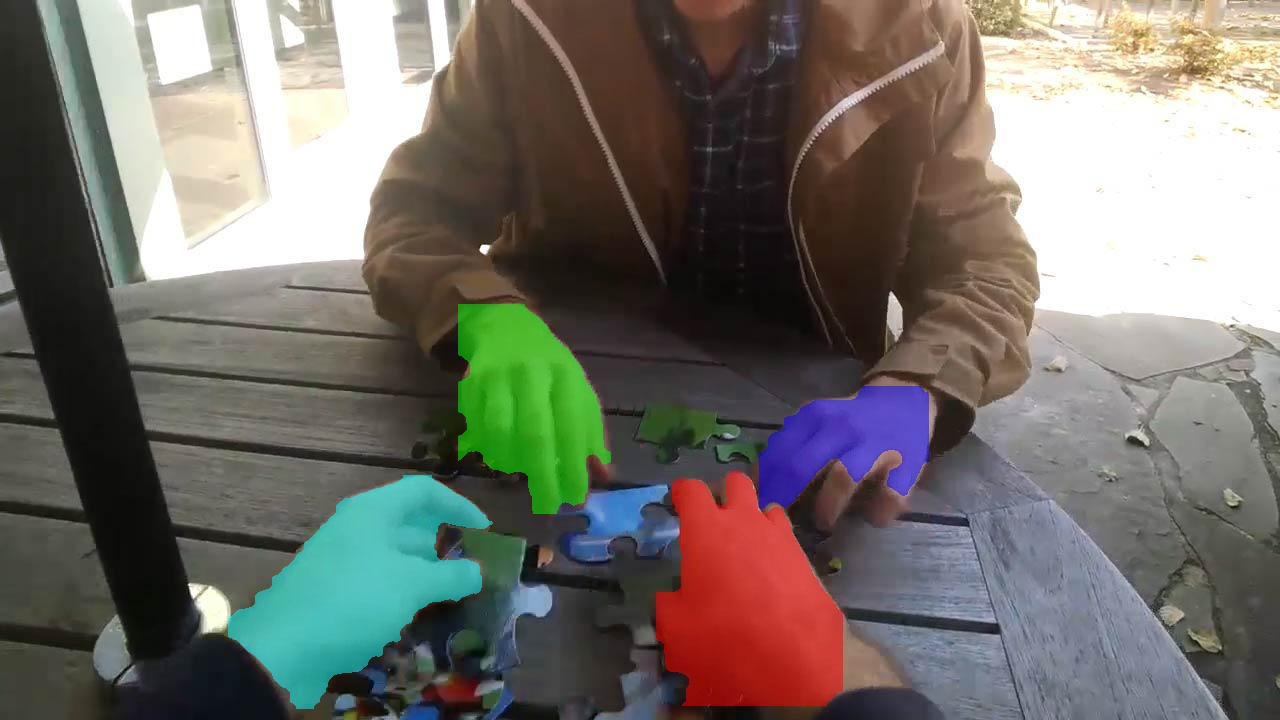
\includegraphics[width=\textwidth]{images/handSegmentation/14.jpg}
        \caption{14.jpg}
        
    \end{subfigure}
    \hfill
    \begin{subfigure}[b]{0.3\textwidth}
        \centering
        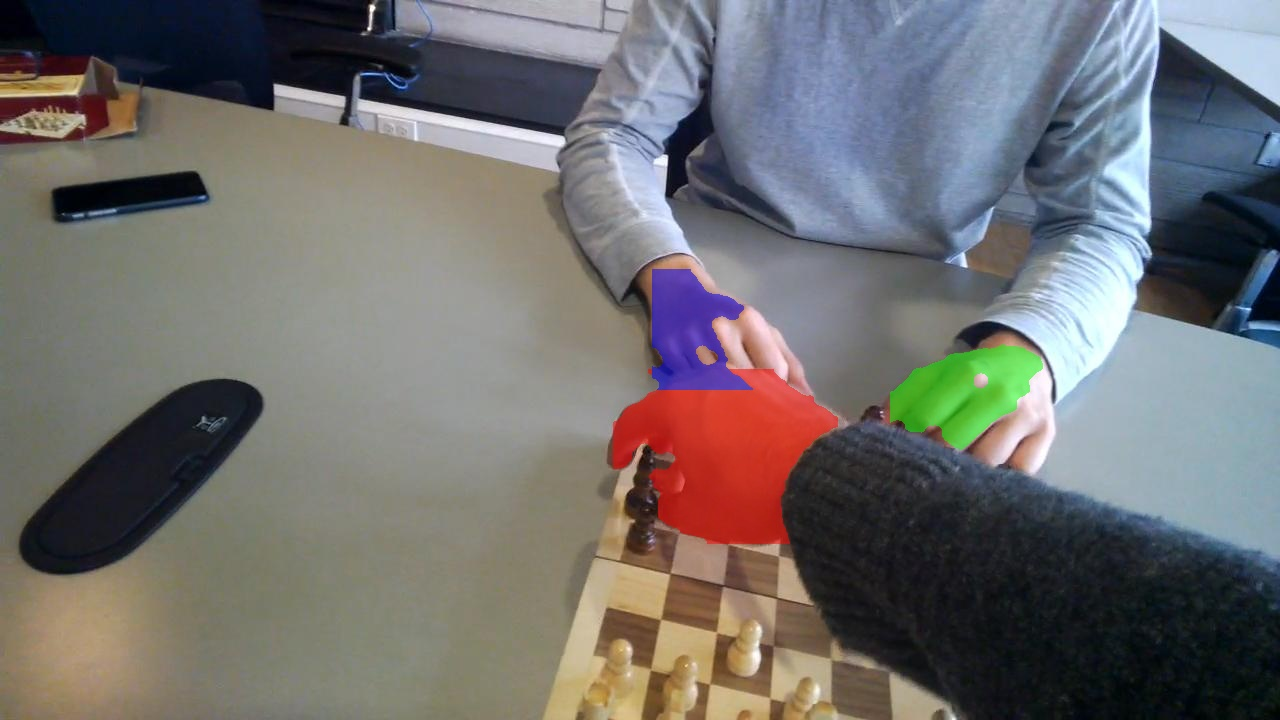
\includegraphics[width=\textwidth]{images/handSegmentation/15.jpg}
        \caption{15.jpg}
       
    \end{subfigure}

    \caption{Segmentation on dataset samples 01-15}
       
\end{figure}



\begin{figure}[!h]
    \centering

    \begin{subfigure}[b]{0.3 \textwidth}
        \centering
        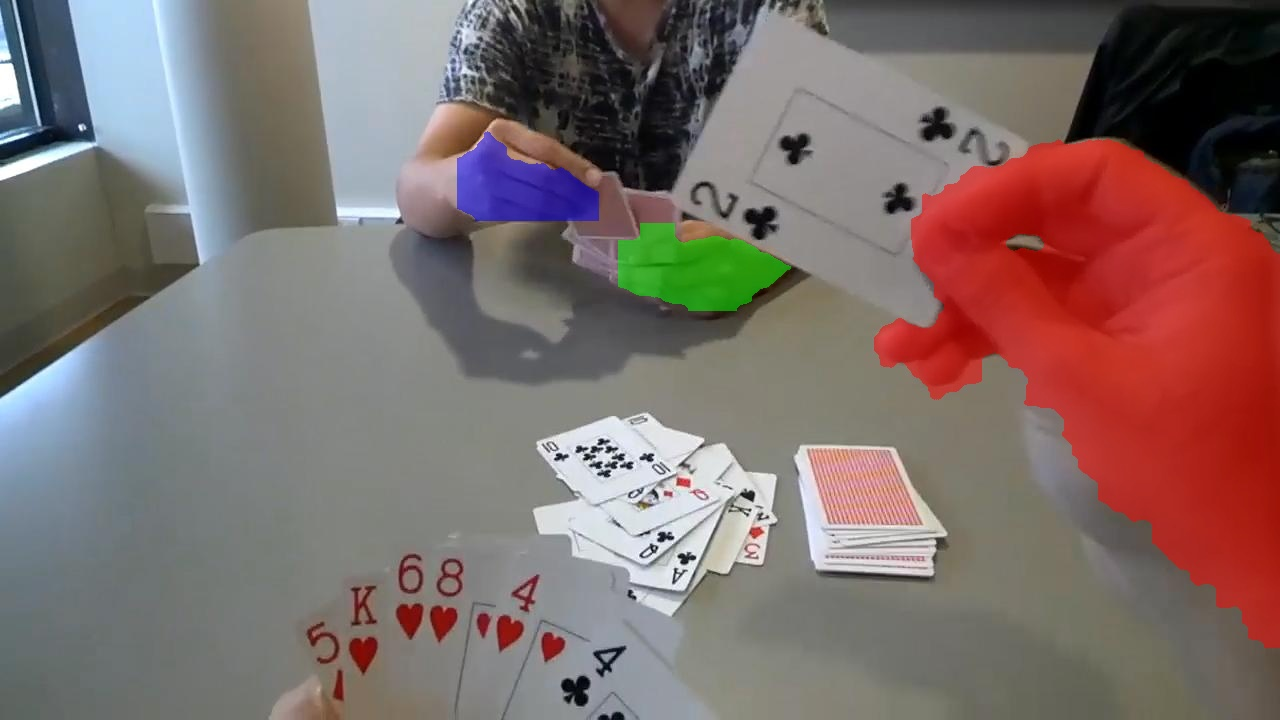
\includegraphics[width=\textwidth]{images/handSegmentation/16.jpg}
        \caption{16.jpg}
        
    \end{subfigure}
    \hfill
    \begin{subfigure}[b]{0.3\textwidth}
        \centering
        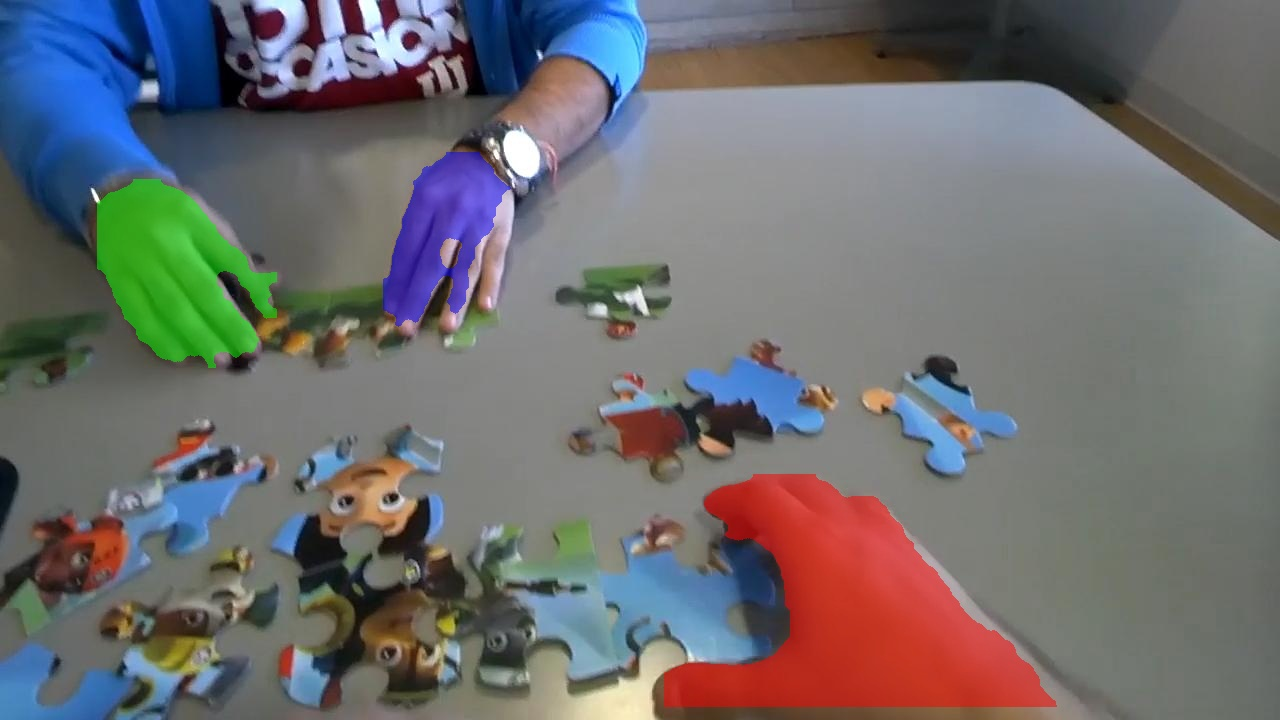
\includegraphics[width=\textwidth]{images/handSegmentation/17.jpg}
        \caption{17.jpg}
        
    \end{subfigure}
    \hfill
    \begin{subfigure}[b]{0.3\textwidth}
        \centering
        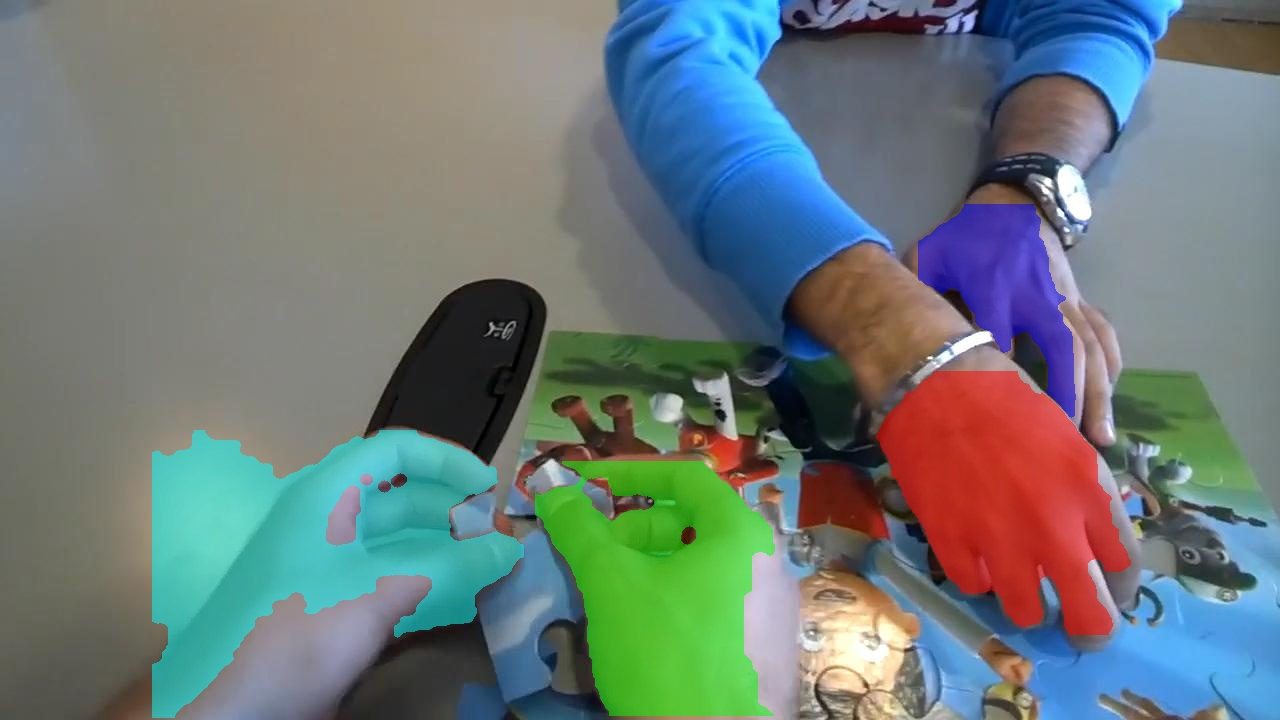
\includegraphics[width=\textwidth]{images/handSegmentation/18.jpg}
        \caption{18.jpg}
        
    \end{subfigure}
       
    \begin{subfigure}[b]{0.3 \textwidth}
        \centering
        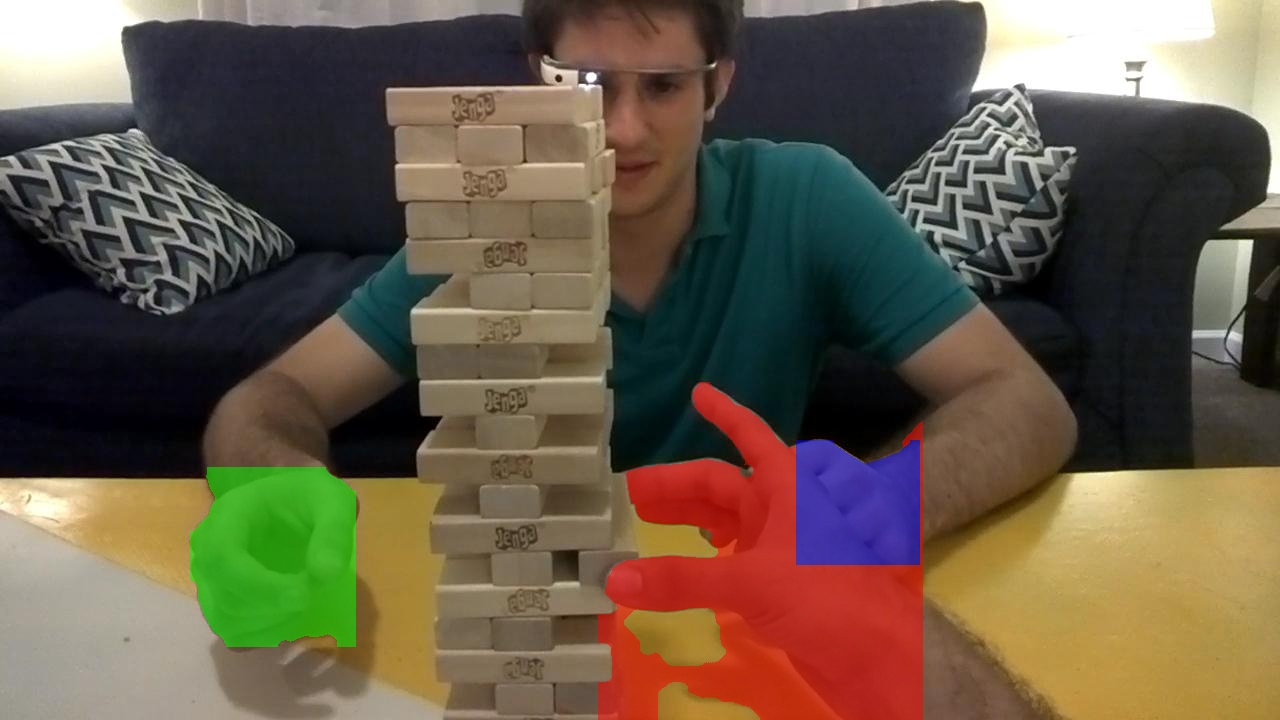
\includegraphics[width=\textwidth]{images/handSegmentation/19.jpg}
        \caption{19.jpg}
        
    \end{subfigure}
    \hfill
    \begin{subfigure}[b]{0.3\textwidth}
        \centering
        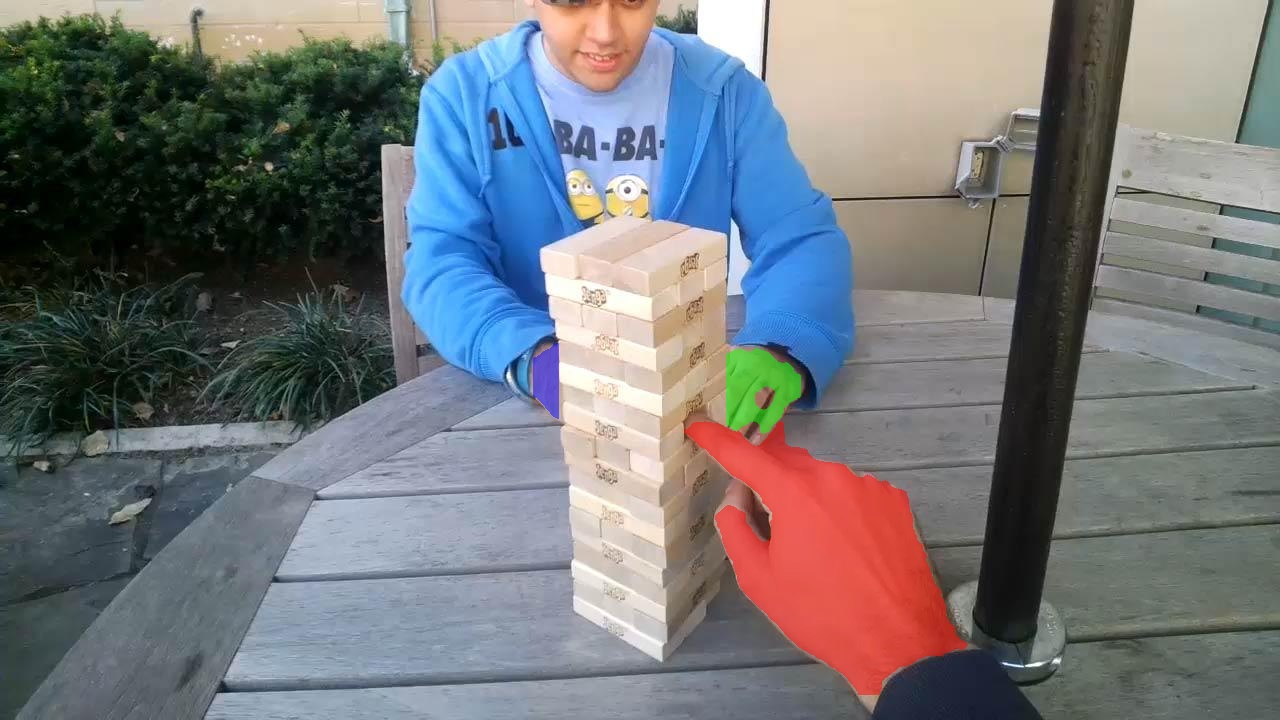
\includegraphics[width=\textwidth]{images/handSegmentation/20.jpg}
        \caption{20.jpg}
        
    \end{subfigure}
    \hfill

    \caption{Segmentation on dataset samples 16-20}
\end{figure}

\begin{table}[h!]
    \centering
    \begin{tabular}{ccc}
    \rowcolor[HTML]{BCBCBC} 
    \multicolumn{1}{l}{\cellcolor[HTML]{BCBCBC}{\color[HTML]{000000} \textbf{Image}}} & \multicolumn{1}{l}{\cellcolor[HTML]{BCBCBC}{\color[HTML]{000000} \textbf{Accuracy}}} & \multicolumn{1}{l}{\cellcolor[HTML]{BCBCBC}\textbf{ROIs accuracy}}                                                                     \\ \hline
    \multicolumn{1}{|c|}{01.jpg}                                                      & \multicolumn{1}{c|}{0.991249}                                                     & \multicolumn{1}{c|}{0.838454}                       \\ \hline
    \multicolumn{1}{|c|}{02.jpg}                                                      & \multicolumn{1}{c|}{0.995158}                                                     & \multicolumn{1}{c|}{0.890629}                       \\ \hline
    \multicolumn{1}{|c|}{03.jpg}                                                      & \multicolumn{1}{c|}{0.995188}                                                     & \multicolumn{1}{c|}{0.90071}                       \\ \hline
    \multicolumn{1}{|c|}{04.jpg}                                                      & \multicolumn{1}{c|}{0.99469}                                                     & \multicolumn{1}{c|}{0.851065}                       \\ \hline
    \multicolumn{1}{|c|}{05.jpg}                                                      & \multicolumn{1}{c|}{0.992398}                                                     & \multicolumn{1}{c|}{0.868971}                       \\ \hline
    \multicolumn{1}{|c|}{06.jpg}                                                      & \multicolumn{1}{c|}{0.98849}                                                     & \multicolumn{1}{c|}{0.88299}                       \\ \hline
    \multicolumn{1}{|c|}{07.jpg}                                                      & \multicolumn{1}{c|}{0.98134}                                                     & \multicolumn{1}{c|}{0.878065}                       \\ \hline
    \multicolumn{1}{|c|}{08.jpg}                                                      & \multicolumn{1}{c|}{0.990567}                                                     & \multicolumn{1}{c|}{0.85287}                       \\ \hline
    \multicolumn{1}{|c|}{09.jpg}                                                      & \multicolumn{1}{c|}{0.993681}                                                     & \multicolumn{1}{c|}{0.729179}                       \\ \hline
    \multicolumn{1}{|c|}{10.jpg}                                                      & \multicolumn{1}{c|}{0.991379}                                                     & \multicolumn{1}{c|}{0.839938}                       \\ \hline
    \multicolumn{1}{|c|}{11.jpg}                                                      & \multicolumn{1}{c|}{0.986956}                                                     & \multicolumn{1}{c|}{0.835139}                       \\ \hline
    \multicolumn{1}{|c|}{12.jpg}                                                      & \multicolumn{1}{c|}{0.963344}                                                     & \multicolumn{1}{c|}{0.838872}                       \\ \hline
    \multicolumn{1}{|c|}{13.jpg}                                                      & \multicolumn{1}{c|}{0.98318}                                                     & \multicolumn{1}{c|}{0.85017}                       \\ \hline
    \multicolumn{1}{|c|}{14.jpg}                                                      & \multicolumn{1}{c|}{0.974145}                                                     & \multicolumn{1}{c|}{0.836776}                       \\ \hline
    \multicolumn{1}{|c|}{15.jpg}                                                      & \multicolumn{1}{c|}{0.982184}                                                     & \multicolumn{1}{c|}{0.770748}                       \\ \hline
    \multicolumn{1}{|c|}{16.jpg}                                                      & \multicolumn{1}{c|}{0.950827}                                                     & \multicolumn{1}{c|}{0.786552}                       \\ \hline
    \multicolumn{1}{|c|}{17.jpg}                                                      & \multicolumn{1}{c|}{0.979173}                                                     & \multicolumn{1}{c|}{0.877487}                       \\ \hline
    \multicolumn{1}{|c|}{18.jpg}                                                      & \multicolumn{1}{c|}{0.927559}                                                     & \multicolumn{1}{c|}{0.762616}                       \\ \hline
    \multicolumn{1}{|c|}{19.jpg}                                                      & \multicolumn{1}{c|}{0.959747}                                                     & \multicolumn{1}{c|}{0.682674}                       \\ \hline
    \multicolumn{1}{|c|}{20.jpg}                                                      & \multicolumn{1}{c|}{0.988677}                                                     & \multicolumn{1}{c|}{0.861342}                       \\ \hline
    \end{tabular}
    \caption{Table summarizing pixel accuracy over the whole image and considering only ROIs}
    \end{table}


\clearpage


\section{Failed attempts}

For the detection module, we first tried using a simple CNN from scratch and train it as a simple classifier, to then scan the entire image
using a pre-fixed sized window and classify it as a hand or notHand. This method was not successful, as the results were not very good: the model
in fact suffering from serious overfitting and the detection took way too long for it to be a viable solution.
We then trained different CNN configurations, but all of them failed to perform the detection in a reasonable amount of time, and also 
the results were very sensible to the chosen size of the window. 

Next we tried to implement the detection using \textit{haar} features, which were not successful either, as the trained model
was again suffering from overfitting and heavy noise sensibility: the haar features performed reasonably well and within a decent amount
of processing time, but as soon as we tried images that did not come from the egohands dataset the results got much worse.

Finally the last thing we tried was to train and use two CNN's in parallel and perform the classification using the output of both.
The first CNN was trained as the first one on an enhanced dataset w.r.t. the original one, and it was trained using the segmented hand images;
the second one was trained on a dataset containing the same images onto which we applied a line detection algorithm: for that we recycled the canny and 
hough transform algorithm we used in one of the laboratories during the course. The results were decent enough, but there was still the problem of running time,
especially since when we deal with 1280x720 images.

For the coarse hand segmentation with skin color detection we tried to use also the HSV color space, but it performed too selective filtering.

We also tried to apply Mean-Shift to the whole image, with unusable computation time.

\section{Final Considerations}
For the hand detection module, the usage of multiple CNN's to attempt to detect and classify hands or any type of object made us realize just 
how sensible the results depend on the dataset we used to train the different nets: most of them worked only if the detection window was the same 
as the one used for training, others suffered from extreme overfitting and noise sensitivity. It is not surprising that even 
the results from the implement YOLO model, which was the most efficient one we tried, still ended up with some overfitting from adopting
mainly one single dataset. 

The main improvement on the hand detection algorithm is then the creation and usage of a more diverse dataset to train the CNN's, in order to avoid phenomenon.
As for the rest of the first module it works very well on the Benchmark images, in fact we do not have one single detection score which is under 85\%, 
and also thanks to the usage of the tensorflow library and a discrete GPU the algorithm revealed to be very fast. The main reason for this efficiency, however,
is the YOLO model architecture we decided to adopt for our detector: thanks to optimized layers and configuration the search for the ROI's inside the image
was extremely fast compared to any other CNN we used thus far.

Considering the hand segmentation module the main concern is the runtime speed, really not suitable for realtime application. On the other hand accuracy shows 
very good results. I can think about two solutions for the runtime speed:
\begin{itemize}
    \item Port the Mean shifted algorithm to GPU hardware
    \item Avoid meanshift and rely only on coarse detection (very fast, but pretty inaccurate)
\end{itemize}

\end{document}